% =====================================================================
%  The zeta(9) first-round attack: a faithful reconstruction of the
%  current proof state (proof-state audit, not a proof).
%
%  Sources: missions/zeta9/{status.md,report.md,research/*.md,verification/*}
%           missions/zeta7/{status.md,research/analytic-foundations.md}
%  Compile: pdflatex (twice, for hyperref); TikZ required for the DAGs.
% =====================================================================
\documentclass[11pt]{article}

\usepackage[margin=1in]{geometry}
\usepackage{amsmath,amssymb,amsthm}
\usepackage{booktabs}
\usepackage{array}
\usepackage{longtable}
\usepackage[hidelinks]{hyperref}
\usepackage{xcolor}
\usepackage{tikz}
\usetikzlibrary{arrows.meta,positioning,calc}
\usepackage{enumitem}

\definecolor{okgreen}{RGB}{0,110,60}
\definecolor{numblue}{RGB}{0,70,160}
\definecolor{heugrey}{RGB}{110,110,110}
\definecolor{gapred}{RGB}{170,20,20}

\newcommand{\stR}{\textcolor{okgreen}{\textbf{R}}}
\newcommand{\stC}{\textcolor{okgreen}{\textbf{R$^{*}$}}}
\newcommand{\stM}{\textcolor{numblue}{\textbf{M}}}
\newcommand{\stN}{\textcolor{numblue}{\textbf{N}}}
\newcommand{\stH}{\textcolor{heugrey}{\textbf{H}}}
\newcommand{\stO}{\textcolor{gapred}{\textbf{OPEN}}}
\newcommand{\Z}{\mathbb{Z}}
\newcommand{\Q}{\mathbb{Q}}
\newcommand{\dd}{\,\mathrm{d}}
\newcommand{\vp}{v_p}
\DeclareMathOperator{\lcm}{lcm}

\title{The $\zeta(9)$ first-round attack:\\ a faithful reconstruction of the current proof state}
\author{Proof-state audit prepared for the \texttt{prove2me\_workspace} local research log}
\date{25 September 2026}

\begin{document}
\maketitle

\begin{center}
\fbox{\parbox{0.94\textwidth}{%
\textbf{Status statement (read first).} This document is an \emph{audit of a proof state}, not a
mathematical paper and not a proof. It covers the \textbf{whole} $\zeta(9)$ effort recorded locally:
nine research rounds (2026-09-24), the local roadmap DAG that succeeded them, and their partial
wiring into a private Prove2me mission. \textbf{No proof of the irrationality of $\zeta(9)$ is
claimed here, and none exists in the audited material.} Every item is classified as rigorously proved
(\stR), proved conditionally on a named standard input (\stC), proved modulo an earlier lemma (\stM),
numerically verified only (\stN), heuristic (\stH), or open/unresolved (\stO).
No gap identified below has been repaired, closed, or worked around; where a statement in the
source notes is weaker than it reads, the weaker reading is recorded.
The unconditional conclusion of this audit is at the top of \S\ref{sec:conclusion}:
\textbf{the audited dependencies include at least ten unclosed obligations, therefore no
irrationality statement is asserted, conditionally or otherwise.}}}
\end{center}

\vspace{0.6em}
\tableofcontents

\section{Scope, sources, and the shape of what exists}
\label{sec:scope}

\textbf{Part I} of this note audits the first research round (dated \textbf{2026-09-24}), recorded
under \texttt{missions/zeta9/} (\texttt{report.md}, \texttt{research/*.md},
\texttt{verification/*}). \textbf{Part II} (\S\S\ref{sec:roadmap}--\ref{sec:closure2}) audits the
remaining eight rounds, the local roadmap that succeeded them
(\texttt{roadmap/DAG.md}, \texttt{dag.json}) and the private Prove2me mission built from it
(\texttt{roadmap/platform/}). The corpus contains:

\begin{itemize}[leftmargin=1.4em]
\item \textbf{nine rounds} (round~1 in \texttt{research/}, rounds 2--9 in \texttt{round2/}\dots
      \texttt{round9/}), each with research notes, scripts and an evidence directory;
\item a \textbf{main route} from round~1 based on a rational function with third-order integer poles,
      seventh-order endpoint zeros, and a sixth derivative summed over positive integers, giving a
      rational linear form $L_{n,m}=A_{n,m}\zeta(9)+B_{n,m}$;
\item a \textbf{secondary (Gram) route} from round~1 using a positive weight functional for odd
      arguments, producing polynomials $\Delta_K(X)$ known to be positive definite at $X=\zeta(9)$
      and of exactly known degree;
\item \textbf{later constructions}: higher-order poles with exact elimination of the other odd
      $\zeta$ values (round~2), rational shifts with fixed divisor weights (round~3), an
      all-$n$ nonvanishing theorem for the leading coefficient (round~4), integer polynomial weights
      on $u=t(t+n)$ (round~5), a Smith-form/primitive-multiplier selection principle (round~6), a
      rational connection theorem with an exact determinant (round~7), and two obstructions inside
      the frozen limit model (rounds 8--9);
\item the \textbf{roadmap DAG}: $40$ named nodes ($13$ open, $27$ ``note-proved''), the object list
      $F_n,K_n,D_n,s_{i,n},N_n,g_n,\Delta_n,\mu_n$ and the parameters $\tau=2641/250$, $\gamma$;
\item a \textbf{private Prove2me mission} (\texttt{8195d8fe-\dots}) with an open root theorem, two
      accepted $SKETCH\_ACCEPTED$ root decompositions, eight theorem-level proofs (two general
      reductions, three abstract cores, three wired lemmas) and $40$ milestones.
\end{itemize}

\textbf{Why the audit matters.} The round's own report already says no irrationality proof was
obtained. The purpose here is to say \emph{precisely which local statements are established, in what
sense, and which of them literally cannot lead anywhere}. Two such structural facts stand out. In
Part I: the analytic side produces only \emph{upper} bounds for $|L|$, while the arithmetic side
controls only \emph{denominators}; a decay-to-zero statement requires either a lower bound for $|L|$
or positivity plus a shortage on the normalization side, and neither route has it. In Part II: every
closing statement is a $\forall$ (over all primitive directions, or over infinitely many $n$) and the
corpus contains only five-scale finite certificates; moreover the newest geometric lemma (FQ) is
vacuous --- its five sample points do not even exist as five distinct admissible points --- below
$n\approx1686$, far beyond every parameter ever used.

\textbf{Formal status.} The mission has no Lean definition for any concrete object of the roadmap
($F_n$, $K_n$, Smith data, weighted areas, congruence-lattice minima). Eight platform theorems exist,
all with abstract statements; the note-proved layer (Part I's local results and the roadmap's $27$
nodes) is not formalized. Status \stR{} therefore means ``a written proof exists and I found no error
in it'', not ``formally verified''.

\section{Conventions and the objects}

\paragraph{Conventions.}
Rising Pochhammer: $(x)_r=x(x+1)\cdots(x+r-1)$. Harmonic sums: $H_j^{(r)}=\sum_{i=1}^{j}i^{-r}$,
$H_0^{(r)}=0$. $\vp$ is the $p$-adic valuation. $v_p(n!)=\sum_{k\ge1}\lfloor n/p^k\rfloor$ (Legendre).
$\psi(x)=\log\lcm(1,\dots,\lfloor x\rfloor)$ is Chebyshev's $\psi$; note $\psi$, \emph{not} $\vartheta$
--- the notes record that an earlier draft wrote $\log\lcm=\vartheta$, which was corrected.
$\{x\}=x-\lfloor x\rfloor$. $\zeta(s)=\sum_{k\ge1}k^{-s}$.

\paragraph{Definitions of the main route.}
\begin{longtable}{@{}p{0.055\textwidth}p{0.88\textwidth}@{}}
\toprule
\textbf{Tag} & \textbf{Definition} \\
\midrule
\endfirsthead
\toprule \textbf{Tag} & \textbf{Definition} \\ \midrule
\endhead
D1 & $R_{n,m}(t)=\dfrac{(n!)^3}{(m!)^{14}}\dfrac{\bigl[(t-m)_m\,(t+n+1)_m\bigr]^{7}}{(t)_{n+1}^{3}}$,
      with $n$ a positive \emph{even} integer and $14m\le 3n+1$ (grid uses $m=\alpha n$,
      $\alpha\in\{0,\tfrac1{28},\tfrac1{14},\tfrac3{28},\tfrac17,\tfrac5{28},\tfrac3{14}\}$). \\
D2 & $L_{n,m}=\dfrac{1}{6!}\sum_{k\ge1}R^{(6)}_{n,m}(k)$. \\
D3 & Partial fractions
      $R_{n,m}(t)=\sum_{j=0}^{n}\Bigl(\frac{C_j}{(t+j)^3}+\frac{D_j}{(t+j)^2}+\frac{E_j}{t+j}\Bigr)$,
      with $C_j=(-1)^{m+j}\binom{n}{j}^{3}\binom{j+m}{m}^{7}\binom{n-j+m}{m}^{7}\in\Z$, and
      $D_j=C_ju_j$, $E_j=\tfrac{C_j}{2}(u_j^2+v_j)$ where ($F_j(t)=(t+j)^3R_{n,m}(t)$)
      $u_j=(\log F_j)'(-j)$, $v_j=(\log F_j)''(-j)$; explicitly
      $u_j=10H_j-10H_{n-j}-7H_{j+m}+7H_{n-j+m}$ (first-order harmonics) and
      $v_j=10H_j^{(2)}+10H_{n-j}^{(2)}-7H_{j+m}^{(2)}-7H_{n-j+m}^{(2)}$. \\
D4 & $A_{n,m}=28\sum_{j=0}^n C_j$ and
      $B_{n,m}=-\sum_{j=0}^{n}\bigl(E_jH_j^{(7)}+7D_jH_j^{(8)}+28C_jH_j^{(9)}\bigr)\in\Q$. \\
D5 & $d=\lcm(1,\dots,n+m)$, $d_n=\lcm(1,\dots,n)$, $G=\gcd_{0\le j\le n}|C_j|$,
      \emph{raw} multiplier $t_{n,m}=2d^{9}/G$, \emph{improved} multiplier $t^{\sharp}_{n,m}=d_n^{9}/G$. \\
D6 & Primitive normalization: $D$ = common denominator of $A,B$; $g=\gcd(|DA|,|DB|)$;
      $m_{\mathrm{prim}}=D/g$; $P_{n,m}(X)=m_{\mathrm{prim}}(A_{n,m}X+B_{n,m})\in\Z[X]$ primitive
      (coefficient gcd $1$); finite gap $g_{n,m}=\tfrac1n\log\bigl(t^{\sharp}_{n,m}/m_{\mathrm{prim}}\bigr)\ge0$. \\
D7 & $\Gamma(\alpha)=7\displaystyle\int_{1}^{\infty}\frac{\mathbf 1_{\{x\}+2\{\alpha x\}\ge2}}{x^{2}}\dd x$. \\
D8 & $K_7(z)=\sum_{k\in\Z}(z-k)^{-7}=\tfrac{1}{6!}\frac{\dd^{6}}{\dd z^{6}}\bigl(\pi\cot\pi z\bigr)$;
      contour line $c=m+\tfrac12$;
      $\Phi_\alpha(w)=-14\alpha\log\alpha+10w\log w+7(w{+}1{+}\alpha)\log(w{+}1{+}\alpha)
      -7(w{-}\alpha)\log(w{-}\alpha)-10(w{+}1)\log(w{+}1)$ (principal branches in the upper half-plane);
      $H_\alpha(y)=\Re\Phi_\alpha(\alpha+iy)-2\pi y$, $y\ge0$. \\
\bottomrule
\end{longtable}

\paragraph{Definitions of the Gram route (inherited from \texttt{missions/zeta7}).}
\begin{longtable}{@{}p{0.055\textwidth}p{0.88\textwidth}@{}}
\toprule \textbf{Tag} & \textbf{Definition} \\ \midrule
\endfirsthead
\toprule \textbf{Tag} & \textbf{Definition} \\ \midrule
\endhead
D9  & $w_s(y)=\dfrac{2(2\pi)^{s-1}}{(s-1)!}y^{s}\sum_{\ell\ge1}\ell^{s-1}e^{-2\pi\ell y}$ for odd $s\ge3$;
       at $s=9$: $w_9(y)=\frac{2(2\pi)^8}{8!}y^{9}\sum_{\ell\ge1}\ell^{8}e^{-2\pi\ell y}$ (positive for $y>0$). \\
D10 & $\mu_X$ is the $\Q$-linear functional fixed by $\mu_X(t^{e})=(-1)^eB_{2e+2}(2e+9)!/[8!(2e+2)!]$
       on monomials and by $\mu_X\bigl((t+j^2)^{-1}\bigr)=j^{8}\bigl(X-H_j^{(9)}\bigr)-\tfrac18+\tfrac1{2j}$
       on simple poles. \\
D11 & $D_a(t)=\prod_{j=1}^{a}(t+j^{2})$, $h=K-N$, $P(t)$ of degree $<h$;
       $G_{ij}(X)=\mu_X\!\bigl(D_N(t)^{2q}t^{i+j}/D_K(t)\bigr)$, $\Delta_K(X)=\det G(X)$,
       screening index $r_K=\log P_K(\zeta(9))/K^{2}$. \\
\bottomrule
\end{longtable}

\section{Inventory: every claim, with status and evidence}
\label{sec:inventory}

Status legend: \stR{} written proof, no error found;
\stC{} proved conditional on a named standard input (explicitly flagged);
\stM{} proved only modulo another claim in the same corpus;
\stN{} certified numerically/interval-wise on a finite range, no uniformity;
\stH{} heuristic, not a proof step; \stO{} needed but absent.
"Evidence" gives the file that carries the claim and, where they exist, the archived artifacts.

\subsection{Main route: construction and exact algebra}

\begin{longtable}{@{}p{0.05\textwidth}p{0.50\textwidth}p{0.075\textwidth}p{0.32\textwidth}@{}}
\toprule \textbf{Tag} & \textbf{Statement} & \textbf{Status} & \textbf{Evidence / notes} \\ \midrule
\endfirsthead
\toprule \textbf{Tag} & \textbf{Statement} & \textbf{Status} & \textbf{Evidence / notes} \\ \midrule
\endhead
R1 & Pole/zero structure: $R_{n,m}$ has poles of order $\le3$ exactly at $0,-1,\dots,-n$ and zeros of
     order $7$ at $1,\dots,m$ and at $-n-m,\dots,-n-1$; degrees give
     $R_{n,m}(t)=O(t^{14m-3(n+1)})=O(t^{-2})$. & \stR & \texttt{research/arithmetic.md} \S1;
     re-derived for this audit. \\
R2 & $L_{n,m}$ converges absolutely. & \stR & follows from R1. \\
R3 & The closed form for $C_j$, and $C_j\in\Z$. & \stR & \texttt{arithmetic.md} \S1; reproduced
     for $(n,m)=(2,0)$ in this audit ($C=(1,-8,1)$, $A=-168$). \\
R4 & $\sum_jE_j=0$ (vanishing of the $t^{-1}$ coefficient at infinity). & \stR & \texttt{arithmetic.md} \S1;
     reproduced: $E=(12,-24,12)$, sum $0$ at $(n,m)=(2,0)$. \\
R5 & Reflection: for even $n$, $R_{n,m}(-n-t)=-R_{n,m}(t)$; hence $D_{n-j}=-D_j$ and $\sum_jD_j=0$. & \stR
     & \texttt{arithmetic.md} \S1; reproduced ($D=(-\tfrac92,0,\tfrac92)$). \\
R6 & Six-derivative summation: $L_{n,m}=A_{n,m}\zeta(9)+B_{n,m}$ with D4, the $\zeta(7)$- and
     $\zeta(8)$-coefficients being killed by R4/R5. & \stR & \texttt{arithmetic.md} \S1;
     \emph{independently reproduced} at $(n,m)=(2,0)$: $L=-168\zeta(9)+176.228515625
     =7.89110563021818797780073476895\ldots$, matching the archived exact direct-sum certificate to the
     full $17$-digit accuracy of its enclosure (\S\ref{sec:checks}). \\
\bottomrule
\end{longtable}

\subsection{Main route: integrality and $p$-adic arithmetic}

\begin{longtable}{@{}p{0.05\textwidth}p{0.50\textwidth}p{0.075\textwidth}p{0.32\textwidth}@{}}
\toprule \textbf{Tag} & \textbf{Statement} & \textbf{Status} & \textbf{Evidence / notes} \\ \midrule
\endfirsthead
\toprule \textbf{Tag} & \textbf{Statement} & \textbf{Status} & \textbf{Evidence / notes} \\ \midrule
\endhead
R7  & Elementary integerization: $du_j\in\Z$, $d^{2}v_j\in\Z$, $d^{r}H_j^{(r)}\in\Z$ for $j\le n$,
      hence $t_{n,m}A_{n,m},t_{n,m}B_{n,m}\in\Z$ with $t_{n,m}=2d^{9}/G$. & \stR
      & \texttt{arithmetic.md} \S2; the factor $2$ is retained here, removed in R8. \\
R8  & \textbf{Improved integerization (headline box):} for $m\le3n/14$,
      $t^{\sharp}_{n,m}A_{n,m}\in\Z$ and $t^{\sharp}_{n,m}B_{n,m}\in\Z$ with $t^{\sharp}_{n,m}=d_n^{9}/G$.
      Proof in two steps: (i) the surface factor $2$ is removed using integral binomial Taylor
      coefficients $\binom{e}{2}\in\Z$ for $e\in\Z$; (ii) the harmonic denominator bound drops from
      $n+m$ to $n$ using the $\le1$ prime-power level $P=p^{a}\in(n,n+m]$ (exists since $n+m<2n$), the
      indicator interval $J=[n+m-P+1,\;P-m-1]$ (nonempty, $|J|-P/2>0$, so every residue class mod
      $P/p$ occurs), and the fact that the $a$-th carry layer contributes exactly $7$ to
      $\vp(C_j)-\vp(C_{j'})$. & \stR\ (written) & \texttt{arithmetic.md} \S2.1;
      \emph{conclusion independently verified} for this audit on
      $(n,m)=(56,0),(56,2),(112,4),(224,8),(224,48)$: $G$ and $d$ recomputed from scratch match the
      records, $t^{\sharp}A\in\Z$, $t^{\sharp}B\in\Z$, and $t^{\sharp}/m_{\mathrm{prim}}$ equals the
      archived integer. \textbf{Caveat: the written proof is a sketch; the carry bookkeeping is the
      least-protected step of the whole arithmetic core (\S\ref{sec:gaps}, G1.2).} \\
R9  & Consistency of the two multipliers: $t_{n,m}/t^{\sharp}_{n,m}=2(d/d_n)^{9}\in\Z_{>0}$. & \stR
      & \texttt{arithmetic.md} \S2.1. \\
R10 & Minimality of the primitive scale: if $tF\in\Z[X]$ for a positive rational $t$, then
      $t/m_{\mathrm{prim}}\in\Z_{>0}$; hence no choice of clearing convention can make any
      already-computed $P$ smaller. & \stR & \texttt{arithmetic.md} \S3 (B\'ezout on the two
      primitive coefficients). \\
R11 & Exact valuations: $\vp(C_j)=3\vp(n!)+7\vp((j+m)!)+7\vp((n-j+m)!)-10\vp(j!)-10\vp((n-j)!)-14\vp(m!)$,
      and $G\mid C_0=\pm\binom{n+m}{m}^{7}$ so all prime divisors of $G$ are $\le n+m$. & \stR
      & \texttt{arithmetic.md} \S4. Re-checked here for $(n\le60,\ \text{all }m,\ p\le n,\ j\in\{0,n/3,n\})$. \\
R12 & \textbf{Large-prime formula:} if $p^{2}>n+m$ and $n\ge2m$, then with $r=n\bmod p$, $s=m\bmod p$,
      $\vp(G)=7\cdot\mathbf 1_{r+2s\ge 2p-1}$. & \stR & \texttt{arithmetic.md} \S5 (case split $p\le n$
      / $p>n$, carry formulas for the three binomials). Finite supports: the notes' own check
      ($818$ parameters, $15\,687$ prime terms, even $n\le120$) and, for this audit, a re-check on
      $216$ parameters / $1\,951$ prime terms with $n\le60$, $0$ failures. \\
R13 & Small primes: $0\le\nu_p:=\vp(G)\le\vp(C_0)\le7\lfloor\log_p(n+m)\rfloor$ and
      $\sum_{p\le\sqrt{n+m}}\nu_p\log p=O(\sqrt n\log n)=o(n)$; the only possible discrepancy between the
      exact large-prime threshold and the continuous floor condition is $r+2s=2p-1$, i.e.\ $p\mid n+2m+1$,
      contributing at most $7\log(n+2m+1)=o(n)$. & \stC & \texttt{arithmetic.md} \S6; conditional on
      $\psi(x)\sim x$ (PNT). Note $\lcm=\psi$ (all prime powers), as corrected. \\
R14 & $\log G=7\sum_{p\le n}\mathbf 1_{\{n/p\}+2\{m/p\}\ge2}\log p+o(n)$ along $m=\alpha n$. & \stC
      & \texttt{arithmetic.md} \S6 (PNT, finite breakpoints for $p/n\ge\varepsilon$, then
      $\varepsilon\downarrow0$). \\
R15 & $\displaystyle\lim\frac{\log G}{n}=\Gamma(\alpha)$, \quad
      $\displaystyle\lim\frac{\log t_{n,m}}{n}=9(1+\alpha)-\Gamma(\alpha)$, \quad
      $\displaystyle\lim\frac{\log t^{\sharp}_{n,m}}{n}=9-\Gamma(\alpha)$. & \stC
      & \texttt{arithmetic.md} \S6; PNT again. \textbf{These are limits of the \emph{multipliers that
      were proved valid}, not of $m_{\mathrm{prim}}$} (see G1.1). \\
R16 & $0\le\Gamma(\alpha)\le14\alpha$ (support of the indicator lies in $[1/(2\alpha),\infty)$).
      Consequently the raw asymptotic cost is $\ge9-5\alpha\ge111/14$ and the improved one is
      $\ge9-14\alpha\ge6$ on $0<\alpha\le3/14$. & \stR & \texttt{arithmetic.md} \S6;
      re-verified numerically for the six grid values (\S\ref{sec:checks}). \\
R17 & Rational interval enclosures for $\Gamma(\alpha)$ (period decomposition of the indicator,
      outward rounding on a $10^{-32}$ grid, explicit tail bound
      $\frac{\ell}{b^{2}(R+1)}\le\int_{Rb}^{\infty}\le\frac{\ell}{b^{2}}(\frac1R+\frac1{R^{2}})$).
      & \stN & \texttt{verification/arithmetic-improved-certificates.json};
      values $\Gamma\in[0.14171563,0.14171565],\dots,[0.85210820,0.85210822]$; all six reproduced
      independently for this audit (\S\ref{sec:checks}). \\
\bottomrule
\end{longtable}

\subsection{Main route: contour identity and analytic upper bound}

\begin{longtable}{@{}p{0.05\textwidth}p{0.50\textwidth}p{0.075\textwidth}p{0.32\textwidth}@{}}
\toprule \textbf{Tag} & \textbf{Statement} & \textbf{Status} & \textbf{Evidence / notes} \\ \midrule
\endfirsthead
\toprule \textbf{Tag} & \textbf{Statement} & \textbf{Status} & \textbf{Evidence / notes} \\ \midrule
\endhead
R18 & \textbf{Exact contour identity:} for $c\in(m,m+1)$, in particular $c=m+\tfrac12$,
      $L_{n,m}=-\dfrac{1}{2\pi i}\displaystyle\int_{c-i\infty}^{c+i\infty}R_{n,m}(z)K_7(z)\dd z$.
      The right-closing rectangle is clockwise; its far edge vanishes since $R=O(z^{-2})$ and its
      horizontal edges because $K_7$ decays exponentially off the real axis; the enclosed residues are
      $\mathrm{Res}_{z=k}RK_7=R^{(6)}(k)/6!$ for $k\ge m+1$, the first $m$ of which vanish. & \stR
      & \texttt{research/analytic.md} \S\S1--2. \textbf{Orientation sign independently re-checked for
      this audit} at $(n,m)=(2,0)$ by direct numerical contour integration: $I=-49.5812789531890297\,i$
      and $-I/(2\pi i)=L=7.89110563021818798$, so the minus sign in (C1) is correct. \\
R19 & Kernel facts: $\sum_{\ell\ge1}\ell^{6}q^{\ell}=\frac{q(1+57q+302q^{2}+302q^{3}+57q^{4}+q^{5})}{(1-q)^{7}}$
      (Eulerian numerator sums to $360$, giving principal part $(z-k)^{-7}$), hence for $\Im z>0$
      $K_7(z)=i\frac{(2\pi)^{7}}{720}\sum_{\ell\ge1}\ell^{6}q^{\ell}$ with $q=e^{2\pi iz}$, and on
      $z=m+\tfrac12+iny$ ($y\ge0$) $q=-e^{-2\pi ny}$ so $|K_7(z)|\le(2\pi)^{7}e^{-2\pi ny}$ and the
      leading phase is $-i$ times a positive constant. & \stR & \texttt{analytic.md} \S2;
      re-derived here (Eulerian numbers $\{1,57,302,302,57,1\}$ for order $6$, numerator sum $360$). \\
R20 & Stirling phase: with $z=nw$, $\Phi_\alpha$ as in D8 gives
      $\log|R|=\frac1n\Re\Phi_\alpha(w)+O_\alpha(1)$ at leading order, and the $n\log n$ coefficient
      cancels exactly: factorial prefactor $3-14\alpha$, products $14\alpha-3$. & \stR
      & \texttt{analytic.md} \S3. Re-derived here. \\
R21 & \textbf{Uniform shifted-Riemann-sum estimate:} putting $\delta=1/(2n)$, $x=\alpha+\delta$,
      $\log|R_{n,m}(m+\tfrac12+iny)|\le n\Re\Phi_\alpha(x+iy)+O_\alpha(\log n)$, \emph{uniformly} in
      $y\ge0$; the replacement of the shifted line by $\Re w=\alpha$ costs $O_\alpha(\log n)$ uniformly
      (for $y\le1$ the only singular term is $-7\log|u-\alpha+iy|$; for $y\ge1$ the four logarithms in
      $\Phi'$ have zero total coefficient and their combination is uniformly bounded). & \stM
      & \texttt{analytic.md} \S3. Proved as a sketch: the four monotonicity comparisons on
      $[0,\alpha]$, $[\alpha,\delta]$ etc.\ are written out, but the implicit constants are not
      tracked. Depends on nothing but Stirling; \emph{no} unresolved external input. \\
R22 & \textbf{Global upper bound:}
      $\displaystyle\limsup_{n\to\infty,\ m=\alpha n}\frac{\log|L_{n,m}|}{n}\le\sup_{y\ge0}H_\alpha(y)$,
      the tail $y\ge Y$ being bounded by $\int_Y^\infty e^{-\pi ny}\dd y$ because
      $14\alpha-3\le0$, and the compact part by an ordinary Laplace upper bound. & \stM
      & \texttt{analytic.md} \S3 (C5). Depends on R18--R21. \textbf{This is an upper bound on $|L|$
      only: it cannot imply nonvanishing, decay, or an asymptotic equality.} \\
R23 & $\Phi'\to H'$: $H'_\alpha(y)=\frac{3\pi}{2}-10\arctan\frac{y}{\alpha}-7\arctan\frac{y}{1+2\alpha}
      +10\arctan\frac{y}{1+\alpha}$, with $H'_\alpha(0)=\frac{3\pi}{2}$ and
      $\lim_{y\to\infty}H'_\alpha(y)=-2\pi$. & \stR & \texttt{analytic.md} \S3 (C6).
      Re-derived symbolically and re-verified numerically ($|{\rm diff}|\sim10^{-40}$) for this audit. \\
R24 & Sign analysis of $H''$: $H''_\alpha(y)\,(\alpha^{2}+y^{2})((1+2\alpha)^{2}+y^{2})((1+\alpha)^{2}+y^{2})$
      is a quadratic in $x=y^{2}$ whose constant coefficient is negative, whose linear coefficient is
      positive, and whose leading coefficient is exactly $3-14\alpha$; hence $H''$ changes sign exactly
      once $(-)\to(+)$, $H'$ has exactly one positive zero, and that zero is the global maximizer of
      $H_\alpha$. & \stN\ (per $\alpha$), \stR\ (shape) & \texttt{analytic.md} \S3;
      archived coefficients in \texttt{verification/analytic-vertical-bound.json}
      (\texttt{hsecond\_numerator}), leading coefficient $=3-14\alpha$ confirmed for all six values
      ($\tfrac52,2,\tfrac32,1,\tfrac12,0$) --- note it \emph{vanishes} at the endpoint $\alpha=\tfrac3{14}$,
      where the quadratic degenerates and the argument uses the linear root. Independent check in
      \S\ref{sec:checks}. \\
R25 & Certified strict upper bounds for $\sup_{y\ge0}H_\alpha$: each maximizer is bracketed between
      exact dyadic rationals and $H$ is evaluated on the whole bracket with $256$-bit Arb balls.
      & \stN & \texttt{verification/analytic-vertical-bound.json};
      $0.671769718688$, $1.167676972547$, $1.609438937754$, $2.021873399673$, $2.416195251742$,
      $2.798637880122$ (strict uppers). Reproduced to $12$ digits for this audit. \\
R26 & Combined upper-bound constants \emph{(the arithmetic cost $9-\Gamma$ of R15 added to the real
      bound of R22, rounded up)}: $9.530055$, $9.885137$, $10.182811$, $10.443667$, $10.707140$,
      $10.946530$; exact rationals archived. & \stN & \texttt{verification/summary.json}
      (\texttt{proved\_combined\_upper\_bounds}). \textbf{All positive: no negative exponent is
      produced on any setting of the grid.} Re-derived in \S\ref{sec:checks}, with the archived
      rationals verified to dominate $9-\Gamma+\sup H$ and to equal its $6$-decimal ceiling. \\
\bottomrule
\end{longtable}

\subsection{Main route: finite exact-arithmetic evidence}

\begin{longtable}{@{}p{0.05\textwidth}p{0.50\textwidth}p{0.075\textwidth}p{0.32\textwidth}@{}}
\toprule \textbf{Tag} & \textbf{Statement} & \textbf{Status} & \textbf{Evidence / notes} \\ \midrule
\endfirsthead
\toprule \textbf{Tag} & \textbf{Statement} & \textbf{Status} & \textbf{Evidence / notes} \\ \midrule
\endhead
R27 & $21$ linear-form samples ($n=56,112,224$, six positive ratios plus the $m=0$ control): exact
      rational $A,B$, exact $d,G$, primitive integer pair $(a,b)$, and Arb enclosures certifying
      $|P_{n,m}(\zeta(9))|>1$ in every case; signs $10$ positive / $11$ negative; nothing timed out.
      & \stN & \texttt{verification/linear-results.jsonl}, \texttt{linear-coeff/} ($21$ gzipped full
      records), \texttt{linear-audit.json} (independent re-read, re-gcd, re-evaluation:
      $21/21$ pass). \\
R28 & No $n=448$ promotion: no profile met either pre-registered gate (both larger scales $<1$, or
      strictly decreasing $\ell_n$). Best main-grid value $\ell_{224}\approx8.273517$ at $\alpha=\tfrac1{28}$.
      & \stN\ (decision) & \texttt{report.md} \S1; gate evaluation based on the certified intervals. \\
R29 & Three direct-sum certificates $(s,n,m)=(9,2,0),(9,6,1),(9,10,2)$: truncated Taylor expansions of
      $R(k+x)$ summed in exact rationals, whole-tail control by the integral test, intervals excluding
      zero and overlapping the partial-fraction $\zeta$-expression. & \stN
      & \texttt{verification/independent-audit.json} (\texttt{linear\_direct\_sum}). The $(9,2,0)$ case
      was reproduced in this audit to $28$ digits ($7.89110563021818797780073476895\ldots$), i.e.\ to
      the full precision of the archived enclosure. \\
R30 & Finite consistency checks: $21+3$ cases pass exact \texttt{Fraction} tests for
      $t^{\sharp}A,t^{\sharp}B\in\Z$, $t^{\sharp}/m_{\mathrm{prim}}\in\Z_{>0}$, recomputed $C$-gcd and
      agreement with the exact coefficients; per-pole first- and second-order integrality of all pole
      rows ($57/113/225$ rows). & \stN & \texttt{verification/arithmetic-improved-certificates.json},
      \texttt{independent-audit.json} (\texttt{improved\_integerization}). \\
\bottomrule
\end{longtable}

\subsection{Gram route}

\begin{longtable}{@{}p{0.05\textwidth}p{0.50\textwidth}p{0.075\textwidth}p{0.32\textwidth}@{}}
\toprule \textbf{Tag} & \textbf{Statement} & \textbf{Status} & \textbf{Evidence / notes} \\ \midrule
\endfirsthead
\toprule \textbf{Tag} & \textbf{Statement} & \textbf{Status} & \textbf{Evidence / notes} \\ \midrule
\endhead
R31 & The functional: $\mu_X(t^{e})=(-1)^eB_{2e+2}(2e+9)!/[8!(2e+2)!]$ from the gamma integral and
      Euler's even-zeta formula; $\mu_X$ on simple poles from Hermite's formula for the Hurwitz zeta,
      with the recorded sign check that $+1/(2j)$ (not $-1/(2j)$) is correct with $H_j$ (Hurwitz value
      $\zeta(9,j)=\zeta(9)-H_{j-1}^{(9)}$). & \stR & \texttt{missions/zeta7/research/analytic-foundations.md}
      \S1 (equations (1)--(4)); inherited, not re-derived in \texttt{zeta9}. \\
R32 & Positivity and exact degree: at $X=\zeta(9)$ the matrix $G$ is positive definite
      ($c^{T}Gc=\int_0^\infty\frac{D_N(y^{2})^{2q}}{D_K(y^{2})}P(y^{2})^{2}w_9(y)\dd y>0$), and
      $[X]G=V\operatorname{diag}(c_j)V^{T}$ with a square Vandermonde gives
      $\deg_X\Delta_K=h=K-N$ and $\Delta_K(\zeta(9))>0$ for every $K$. & \stR
      & zeta7 \texttt{analytic-foundations.md} \S2 (equations (5)); inherited. \textbf{This is the only
      genuine nonvanishing statement in the corpus, and it is about positivity at finite $K$ --- it
      says nothing about size relative to the denominator.} \\
R33 & Residue-at-infinity form: $B_{ij}=+[t^{-1}]_\infty t^{i+j+4}P(t)/D_K(t)$, whose first possible
      nonzero anti-diagonal is $i+j=K-\deg P-5$ (one earlier than for $s=7$). & \stM
      & \texttt{zeta9/research/analytic.md} \S4; stated with the $s=7$ comparison, index shift not
      re-derived here. \\
R34 & Moment integrality: $w_9$ has $7$ numerator factors $2e+3,\dots,2e+9$; for $p\ge11$ the moments
      $\mu_9(t^{e})$ are $p$-integral for every $e<4p-5$, and at $e=4p-5$ (Bernoulli index $8(p-1)$,
      numerator factors $8p-7,\dots,8p-1$ containing no $p$) von Staudt--Clausen gives valuation
      exactly $-1$. & \stC & \texttt{zeta9/research/analytic.md} \S4; conditional on
      von Staudt--Clausen, and on the $-1$ claim being a \emph{possible}-worst-case statement. The
      threshold count $4p-5$ for $s=9$ (versus $3p-4$ for $s=7$) follows from \#factors $=s-2=7$. \\
R35 & Rank bound: for the unshifted $D_N^{8}$ matrix the first possible polynomial correction sits at
      $i+j=K-8N+4p-5$ and its rank is at most $\min\bigl(h,[K+6N-4p+4]_+\bigr)$. & \stM
      & \texttt{zeta9/research/analytic.md} \S4. Derived by adapting the $s=7$ bound (zeta7
      \texttt{analytic-foundations.md} \S5 (15), which gives $\operatorname{rank}L\le\max(0,K+(2q-2)N-3p+3)$);
      the index shift was \emph{not} re-derived for this audit and shows a $-1$ difference from the
      zeta7 pattern. The note itself calls this a moment-integrality/rank lemma and
      \emph{not a determinant valuation theorem}. \\
R36 & Transfer $s=7\to s=9$: changing $s$ alters only polynomial prefactors of $w_s(K\sqrt t)$, so with
      the same $q,\alpha,h/K$ the leading $K^{2}$ external field and the logarithmic-energy comparison
      are unchanged, while the prime-by-prime integerization cost is \emph{not} transferable (both the
      Bernoulli-moment thresholds and the harmonic-pole valuations change). & \stH
      & \texttt{zeta9/research/analytic.md} \S4 (last paragraph). A structural remark, not a proof; it
      is nevertheless the reason a $\zeta(9)$ Gram claim cannot quote the $\zeta(5)$ paper's
      arithmetic. \\
R37 & Finite Gram evidence: $18$ records at $K=40$ plus $3$ at $K=80$; all $21$ values $>1$; the three
      promoted profiles rise, $r_{40}\to r_{80}$: $1.343774\to1.429423$ ($q=4,N/K=3/20,h/K=1/2$),
      $1.387844\to1.432339$ ($q=5,N/K=3/20$), $1.514384\to1.623551$ ($q=5,N/K=3/40$); regression
      controls reproduce $r_{40}(\zeta(5))=-0.165705667$ and $r_{40}(\zeta(7))=0.766949846$ with
      matching coefficient hashes. & \stN & \texttt{verification/gram-results.jsonl},
      \texttt{gram-manifest.json}, \texttt{independent-audit.json}. Note the $\zeta(5)$ control is the
      only record below one. \\
R38 & Assignment dual certificates covering \emph{all} denominator primes for the best profile at two
      scales; after integer Newton change of basis the extra cost over the primitive multiplier is
      $\log(\mathrm{gap})/K^{2}\approx1.690479$ ($K=40$) and $1.817305$ ($K=80$); the primitive
      polynomial is unchanged. & \stN & \texttt{verification/gram-arithmetic-certificates.json};
      explicitly a finite certificate, not used as an asymptotic bound. \\
R39 & Literature boundary: the family sits in the lineage of Zudilin's derivative linear forms in the
      central variable with parameters $a=3$, $b=7$, $c=1+2\alpha$; the source's $c\ge3$ odd-integer
      domain does not cover this range, hence its $\Pi$ common-factor and saddle theorems are
      \emph{not} invoked. & \stH & \texttt{arithmetic.md} \S7
      (\href{https://arxiv.org/pdf/math/0104249}{Zudilin 2001, \S3--4}). A correct scoping decision;
      it also means no external theorem supplies the missing asymptotics. \\
\bottomrule
\end{longtable}

\subsection{The unclosed obligations (all of them open)}

\begin{longtable}{@{}p{0.05\textwidth}p{0.58\textwidth}p{0.075\textwidth}p{0.22\textwidth}@{}}
\toprule \textbf{Tag} & \textbf{What is needed (and is absent)} & \textbf{Status} & \textbf{Where it would be needed} \\ \midrule
\endfirsthead
\toprule \textbf{Tag} & \textbf{What is needed (and is absent)} & \textbf{Status} & \textbf{Where it would be needed} \\ \midrule
\endhead
T1 & $A_{n,m}\ne0$ (and exclusion of the degenerate case $A=B=0$, which the notes explicitly say must
     be recorded as a degenerate zero case with no primitive scale). & \stO
     & Any use of $P_{n,m}=m_{\mathrm{prim}}(A\zeta(9)+B)$ as a linear form in $\zeta(9)$. Nothing in
     the corpus certifies $A\ne0$; the certified $|P|>1$ does not imply it (a nonzero integer constant
     would do just as well). \\
T2 & Eventual nonvanishing of $L_{n,m}$ along any infinite sequence. & \stO
     & The irrationality criterion; R22 is an upper bound and cannot supply it. \\
T3 & A \emph{lower} bound for $|L_{n,m}|$ (equivalently a main term with a controlled phase, with the
     conjugate contributions shown not to cancel). The saddle equation
     $\Phi'_\alpha(w)+2\pi i=0$ is written down, then explicitly \emph{not} used: exponentiation loses
     the logarithm branch, and root location would give neither dominance nor non-cancellation. & \stO
     & Decay of the integer forms. This is the structural heart of the gap (\S\ref{sec:gaps}, G1.2). \\
T4 & An asymptotic for the \emph{true} primitive multiplier $m_{\mathrm{prim}}$ (or a matching lower
     bound). What is proved is that $m_{\mathrm{prim}}\mid t^{\sharp}$, i.e.\ an \emph{upper} bound
     $\log m_{\mathrm{prim}}/n\le9-\Gamma(\alpha)$. & \stO
     & The arithmetic side of the exponent comparison. \\
T5 & Assembly: $0<|P_{n,m}(\zeta(9))|\le e^{-cn}$ for some $c>0$ and all large $n$ along a sequence. & \stO
     & The irrationality conclusion itself. \\
T6 & A phased saddle main term for the Gram determinant; uniformity of the $O(K\log K)$ terms and of
     the circle-regularization error; and the combined-exponent inequality
     $\limsup K^{-2}\log m_K<-[\,\lambda M-I(\rho)+C^{*}(q,\alpha)]$ of zeta7 \S4 (13). & \stO
     & The Gram route's criterion. Additionally the potential certificate $M=-1329/200$ of the
     $\zeta(5)$ paper is \emph{imported and not independently certified} (zeta7 says so explicitly), and
     the local-mass hypothesis needed for the $O(\sqrt\varepsilon)$ circle error is listed as an
     \emph{assumption}. \\
T7 & Any formalization. & \stO & \texttt{status.md}: no Lean work has been started. \\
\bottomrule
\end{longtable}

\section{Dependency DAG toward the irrationality of $\zeta(9)$}
\label{sec:dag}

Green boxes are closed (\stR/\stC), blue are finite/numerical (\stN), grey are heuristic (\stH), red
dashed are open (\stO). Solid arrows are logical dependencies; the red dashed arrows are the
directions in which the corpus contains \emph{no} implication at all.

\begin{center}
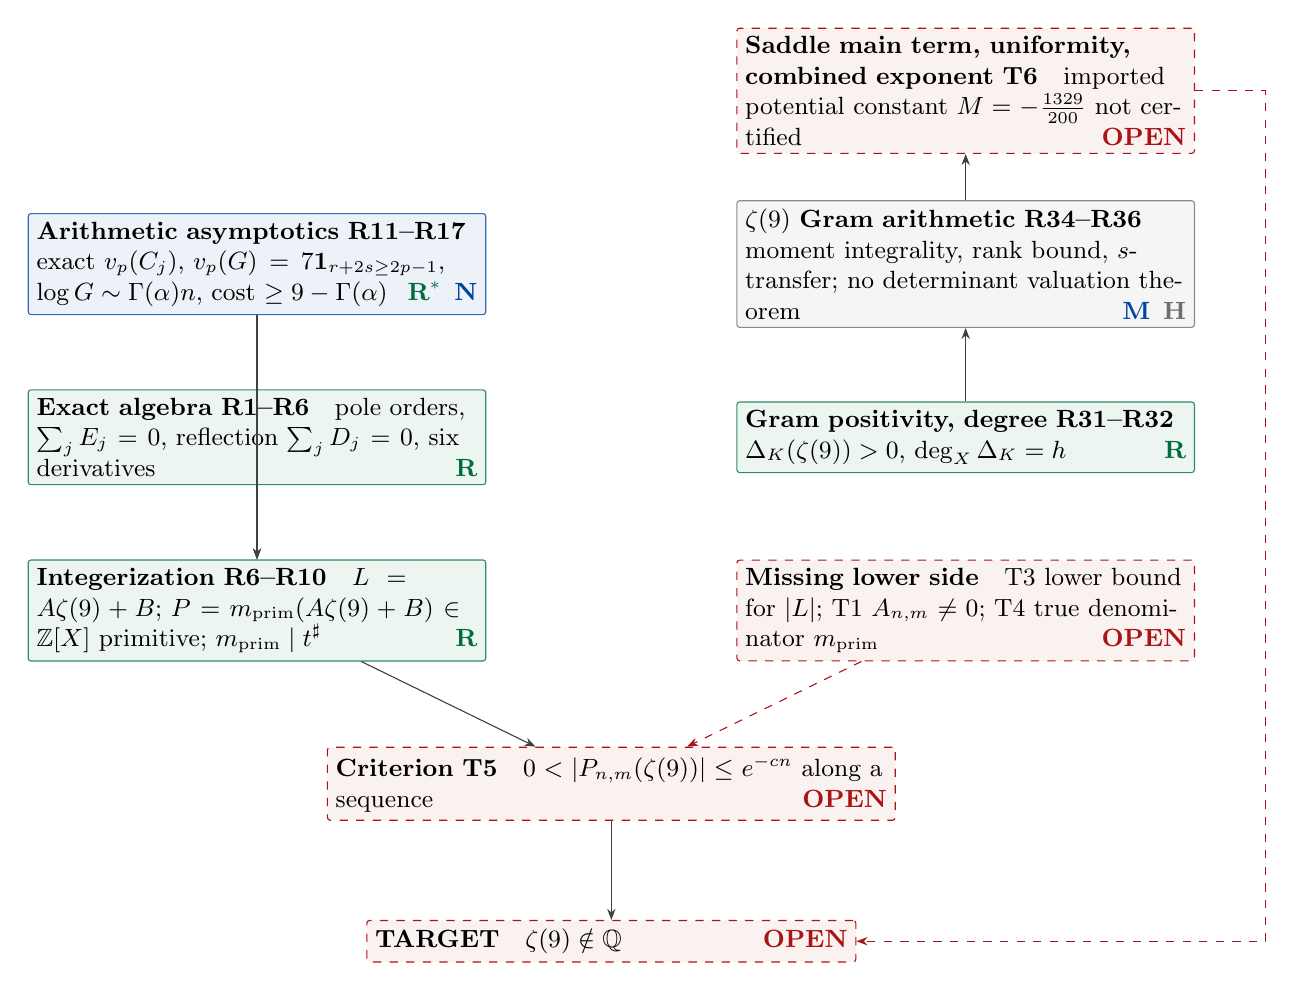
\begin{tikzpicture}[
  font=\small,
  box/.style={draw, rounded corners=1pt, inner sep=3pt, align=left},
  ok/.style={box, draw=okgreen!80, fill=okgreen!7},
  num/.style={box, draw=numblue!80, fill=numblue!7},
  heu/.style={box, draw=heugrey!80, fill=heugrey!7},
  gap/.style={box, draw=gapred, dashed, fill=gapred!6},
  ar/.style={-{Stealth[length=4pt]}, draw=black!75},
  mr/.style={-{Stealth[length=4pt]}, draw=gapred, dashed}
]
% ---- nodes ------------------------------------------------------------------
\node[gap, text width=6.0cm] (target) at (7.5, 0.9)
  {\textbf{TARGET}\quad $\zeta(9)\notin\Q$ \hfill \stO};
\node[gap, text width=7.0cm] (crit) at (7.5, 2.9)
  {\textbf{Criterion T5}\quad $0<|P_{n,m}(\zeta(9))|\le e^{-cn}$ along a sequence \hfill \stO};

\node[ok, text width=5.6cm] (int) at (3.0, 5.1)
  {\textbf{Integerization R6--R10}\quad $L=A\zeta(9)+B$; $P=m_{\mathrm{prim}}(A\zeta(9)+B)\in\Z[X]$
   primitive; $m_{\mathrm{prim}}\mid t^{\sharp}$ \hfill \stR};
\node[gap, text width=5.6cm] (lb) at (12.0, 5.1)
  {\textbf{Missing lower side}\quad T3 lower bound for $|L|$; T1 $A_{n,m}\ne0$;
   T4 true denominator $m_{\mathrm{prim}}$ \hfill \stO};

\node[ok, text width=5.6cm] (alg) at (3.0, 7.3)
  {\textbf{Exact algebra R1--R6}\quad pole orders, $\sum_jE_j=0$, reflection $\sum_jD_j=0$,
   six derivatives \hfill \stR};
\node[num, text width=5.6cm] (arith) at (3.0, 9.5)
  {\textbf{Arithmetic asymptotics R11--R17}\quad exact $\vp(C_j)$,
   $\vp(G)=7\mathbf 1_{r+2s\ge2p-1}$, $\log G\sim\Gamma(\alpha)n$, cost $\ge9-\Gamma(\alpha)$
   \hfill \stC\, \stN};

\node[ok, text width=5.6cm] (Gram) at (12.0, 7.3)
  {\textbf{Gram positivity, degree R31--R32}\quad $\Delta_K(\zeta(9))>0$,
   $\deg_X\Delta_K=h$ \hfill \stR};
\node[heu, text width=5.6cm] (gramar) at (12.0, 9.5)
  {\textbf{$\zeta(9)$ Gram arithmetic R34--R36}\quad moment integrality, rank bound,
   $s$-transfer; no determinant valuation theorem \hfill \stM\, \stH};
\node[gap, text width=5.6cm] (saddle) at (12.0, 11.7)
  {\textbf{Saddle main term, uniformity, combined exponent T6}\quad imported potential constant
   $M=-\tfrac{1329}{200}$ not certified \hfill \stO};

% ---- edges ------------------------------------------------------------------
\draw[ar] (alg) -- (int);
\draw[ar] (arith) -- (int);
\draw[ar] (int) -- (crit);
\draw[mr] (lb) -- (crit);
\draw[ar] (crit) -- (target);
\draw[ar] (Gram) -- (gramar);
\draw[ar] (gramar) -- (saddle);
\draw[mr] (saddle.east) -- +(0.9,0) |- (target.east);
\end{tikzpicture}
\end{center}

\noindent\textbf{Standard inputs} (used \stC, drawn as dotted edges in the text list below, omitted
from the picture for legibility): PNT $\psi(x)\sim x$ (feeds R13--R15), Legendre's formula (R11),
von Staudt--Clausen (R34), Euler's even-zeta formula (R31).

\noindent\textbf{Edge list (text form, for grep-ability).}
\begin{quote}\ttfamily\small
target <- crit;\newline
crit <- int, lb;\newline
int <- alg(R1-R6), arith(R11-R17);\newline
arith <- [pnt, psi~x];\quad int <- [Legendre, von Staudt-Clausen];\newline
lb <- (nothing: no lower-bound mechanism exists);\newline
target <- saddle (Gram branch only);\newline
saddle <- gramar(R34-R36), [imported: potential certificate M; assumption: local mass estimate];\newline
gramar <- Gram(R31-R32);\newline
T1 <- (nothing);\quad T4 <- (nothing);\quad T7 <- (nothing).
\end{quote}

\noindent\textbf{Reading of the DAG.} The main route has \emph{two} red edges and both are on the
`crit' row: it closed the algebra, the integrality and the arithmetic-asymptotic side, and it
produced a genuine analytic upper bound; but the inequality it needs points the other way (T3), and
the denominator it needs to control is not the one it controlled (T4). The Gram route replaces the
missing lower bound by positivity (R32), but then has to pay for it: the determinant grows like
$e^{r_KK^{2}}$ with $r_K\approx1.34$--$1.62$ (R37), so decay requires the normalization multiplier to
be smaller than $e^{-r_KK^{2}}$ --- precisely the inequality (T6) that is open, and whose $\zeta(9)$
arithmetic is declared non-transferable from the $\zeta(5)$ paper (R36).

\section{Gap audit, by category}
\label{sec:gaps}

\subsection{Integrality and denominator bounds}
\begin{itemize}[leftmargin=1.4em]
\item \textbf{Closed (with one caveat):} R3--R12, R30. The headline statement
      $d_n^{9}A/G,\,d_n^{9}B/G\in\Z$ (R8) is a real, non-trivial improvement over the elementary
      $2d^{9}/G$ (R7) and R9 shows the two are consistent.
\item \textbf{G1.1 (open).} The asymptotics R15 are limits of \emph{valid but possibly non-optimal}
      multipliers. Since $t^{\sharp}$ is a valid multiplier, $m_{\mathrm{prim}}\mid t^{\sharp}$, so
      $9-\Gamma(\alpha)$ is an \emph{upper} bound for $\lim\log m_{\mathrm{prim}}/n$. The measured
      finite gaps $g_{n,m}=\frac1n\log(t^{\sharp}/m_{\mathrm{prim}})$ are $0.86,0.71,0.71,0.67,0.62,0.74$
      at $n=224$ and show no sign of vanishing; their limit is unknown. Therefore the quantity
      $9-\Gamma(\alpha)$ that the report calls ``the arithmetic cost'' is \emph{not} the cost of the
      primitive form, and the derived statements ``cost $\ge9-5\alpha\ge111/14$'' /
      ``$\ge9-14\alpha\ge6$'' (R16) are lower bounds for an upper bound of the true cost. Using them as
      if they were the true cost is a resource-accounting heuristic, not an inequality.
\item \textbf{G1.2 (fragility).} R8's written proof is a sketch, not machine-checked. Its delicate part
      is the claim that the top prime-power level contributes exactly $7$ to $\vp(C_j)-\vp(C_{j'})$
      for the chosen $j'\equiv j \pmod{p^{a-1}}$ in $J$, together with the non-emptiness of $J$
      ($|J|-P/2=n/2-2m+1/2>0$). This audit verified the \emph{conclusion} on five cases
      (including $n=224$) but not the proof. No artifact in the corpus formalizes it.
\item \textbf{G1.3 (Gram).} No determinant valuation theorem exists: the notes say so explicitly
      (R35 is a moment-integrality/rank lemma). Hence the Gram route's normalization cost is known
      only through finite dual certificates (R38), which are not asymptotic.
\end{itemize}

\subsection{Nonvanishing}
\begin{itemize}[leftmargin=1.4em]
\item \textbf{What exists:} finite certified $|P|>1$ on $21$ samples (R27); three direct-sum certificates
      (R29); and the Gram positivity $\Delta_K(\zeta(9))>0$ for every $K$ (R32).
\item \textbf{G2.1 (open).} $A_{n,m}\ne0$ is never asserted (T1). Certified $|P|>1$ does not imply $A\ne0$.
\item \textbf{G2.2 (open).} No eventual nonvanishing (T2). The notes state this in three places; it is
      recorded here so that no reader upgrades ``all $21$ values exceed $1$'' into an asymptotic statement.
\item \textbf{G2.3 (structural).} R22 bounds $|L|$ from \emph{above}. No chain of upper bounds can
      yield nonvanishing or decay, and no lower-bound mechanism (saddle main term, sign of a leading
      term, positivity on the linear-form side) currently exists on the main route. This is the single
      most important structural fact about the round.
\item \textbf{G2.4 (Gram caveat).} Positivity gives nonvanishing but at a price: the certified size
      grows ($r_K>0$, R37), so the required smallness must come entirely from the multiplier side --- open.
\end{itemize}

\subsection{$p$-adic valuation estimates}
\begin{itemize}[leftmargin=1.4em]
\item \textbf{Closed:} the exact formula R11 (all primes, all $j$), the large-prime formula R12
      (hypothesis $p^{2}>n+m$, plus $n\ge2m$ in the $p>n$ branch --- satisfied because $m\le3n/14<n/2$),
      and the crude small-prime bound R13. Note the notes' own warning: one may \emph{not} generally
      interchange $\min_j\sum_k$ with $\sum_k\min_j$; the implementation keeps the correct order and
      cross-checks with an independent integer gcd.
\item \textbf{G3.1 (open).} No valuation statement for the primitive content of $P$, nor for the
      determinant of the Gram matrix. The prime-by-prime structure of the Gram route is explicitly
      declared non-transferable from $s=7$ (R36).
\item \textbf{G3.2 (scope).} R12 is a statement about $G=\gcd_j|C_j|$ (a single integer), not about the
      determinant/correction matrices of the Gram route; conflating them would be an error.
\end{itemize}

\subsection{Asymptotic estimates}
\begin{itemize}[leftmargin=1.4em]
\item \textbf{Closed (conditionally):} R13--R15 (PNT, all prime powers via $\psi$), R17 (rational
      enclosures with explicit tails).
\item \textbf{Closed (as a sketch):} R20--R22. The phase cancellation in R20 is exact; R21's uniformity
      argument is written but the constants are implicit; R22 follows from R18--R21 plus a compact
      Laplace bound and an exponential tail ($14\alpha-3\le0$, so the tail \emph{decays}).
\item \textbf{G4.1 (open).} No asymptotic lower bound for $|L|$; no asymptotic for
      $m_{\mathrm{prim}}$; no saddle evaluation. \emph{Do not read} $\sup_{y\ge0}H_\alpha$ as a decay
      rate --- it is an upper bound for the growth rate of $|L|$.
\item \textbf{G4.2 (inherited).} On the Gram side, the real-value estimate (zeta7 (10)--(12)) requires
      (i) an imported potential certificate that is not independently certified, and (ii) an assumed
      local mass estimate for the $O(\sqrt\varepsilon)$ circle error. Neither is supplied within the
      audited corpus.
\end{itemize}

\subsection{Signs of all exponential constants}
Audited one by one; the sign conventions are \emph{not} a formality here, because a flipping sign in
$H'$ or in the contour identity would change every constant in \S\ref{sec:inventory}.

\begin{itemize}[leftmargin=1.4em]
\item \textbf{Contour orientation (R18).} Verified independently for $(n,m)=(2,0)$ by direct numerical
      integration: $I=\int_{c-i\infty}^{c+i\infty}RK_7 = -49.5812789531890297\,i$ and
      $-\tfrac{1}{2\pi i}I=+7.89110563021818798=L$. So the minus sign in (C1) is \emph{correct}
      (the right-closing rectangle traverses the vertical line upward).
\item \textbf{Kernel phase (R19).} $K_7=i\frac{(2\pi)^7}{720}q(1+57q+302q^2+302q^3+57q^4+q^5)/(1-q)^7$
      with $q=e^{2\pi iz}$: on the upper contour $q=-e^{-2\pi ny}$, so $K_7$ carries phase
      $-i\times(\text{positive})$ and modulus $\le(2\pi)^{7}e^{-2\pi ny}$. The numerator sum $360$
      is what makes the principal part $(z-k)^{-7}$; both facts were re-derived here.
\item \textbf{$H'$ limits (R23):} $H'(0)=+3\pi/2>0$, $H'(\infty)=-2\pi<0$; the sign change is single
      because of R24. The intermediate value $H'(0.1)\approx-7.25$ for $\alpha=\tfrac1{28}$ shows the
      maximizer is genuinely at small $y$, not at the boundary.
\item \textbf{$H''$ leading coefficient (R24):} exactly $3-14\alpha$, i.e.\ $+2.5,+2,+1.5,+1,+0.5,0$
      for the six grid values; verified against the archived rational data. The endpoint
      $\alpha=3/14$ is \emph{degenerate} (coefficient $0$, quadratic becomes linear) and is handled by
      the general root argument, but it is the one place where the shape claim is not uniform.
\item \textbf{$\Gamma$ bounds (R16):} $0\le\Gamma(\alpha)\le14\alpha$ with equality in the upper bound
      never attained on the grid ($\Gamma\le0.853$ against $14\alpha\ge0.5$).
\item \textbf{Sign of the final constants:} every certified number that would have to be negative for a
      conclusion is positive: R25's $\sup H_\alpha\in(0.67,2.80)$, R26's combined bounds
      $\in(9.53,10.95)$, R37's $r_K\in(1.34,1.62)$, R38's gaps $>0$. There is \emph{no} setting of the
      grid in which a negative exponent appears.
\item \textbf{Inherited sign convention (R31):} the $+1/(2j)$ in $\mu_X\bigl((t+j^2)^{-1}\bigr)$ is
      recorded in zeta7 as a sign check that was performed (Hurwitz value vs.\ $H_j$). It is inherited,
      not re-derived in \texttt{zeta9}; the Gram route's positivity depends on it.
\end{itemize}

\subsection{Uniformity of all $O(\cdot)$ terms}
\begin{itemize}[leftmargin=1.4em]
\item \textbf{Uniformity claimed and argued:} R21's $O_\alpha(\log n)$ is claimed uniform in $y\ge0$,
      with the shift $\delta=1/(2n)$ handled by two separate estimates ($y\le1$ via
      $-7\log|u-\alpha+iy|\le7|\log(u-\alpha)|+O_\alpha(1)$; $y\ge1$ via the zero total coefficient of
      the four logarithms in $\Phi'$ --- the total coefficient is $10+7-7-10=0$, checked here).
      R22's tail is claimed uniformly in $n\ge1$ for $Y$ large enough.
\item \textbf{G6.1 (open).} No explicit constants: ``$O_\alpha(\log n)$'' with an unquantified
      $\alpha$-dependent constant is enough for a limsup \emph{only} because the target is a rate, but
      it cannot be turned into a finite-$n$ statement, and the notes are right not to try.
\item \textbf{G6.2 (inherited, open).} The Gram route's $O_{s,q,\alpha,\rho}(K\log K)$ in zeta7 (8)/(12)
      is uniform only under the stated local-mass assumption on the comparison measure; zeta7 lists
      this as an assumption, and the potential certificate is imported. For $s=9$, R36 says the
      leading terms are unchanged but \emph{does not certify} the $O_s$ terms.
\item \textbf{G6.3 (minor, open).} R35's index shift relative to the $s=7$ rank bound differs by one
      unit ($K+6N-4p+4$ vs the pattern's $K+6N-4p+5$); whichever is intended, the bound is
      $\min$-capped by $h$ and no conclusion depends on it, but the line should be re-derived before
      being quoted. Flagged as an unverified adaptation, not as an error.
\end{itemize}

\subsection{Two further structural remarks (not repaired)}
\begin{itemize}[leftmargin=1.4em]
\item \textbf{G7.1.} The two routes are logically independent, and the Gram route inherits an
      unfinished arithmetic program (zeta7's own status is ``no proof of irrationality''), including
      its imported, uncertified potential constant.
\item \textbf{G7.2.} The report's closing judgement --- that the next round should change the structure
      rather than clear more denominators, because the real side can supply at most
      $\sup H_\alpha\lesssim2.80$ against an arithmetic side bounded by $8.15$--$8.86$ --- is a
      \emph{heuristic prioritisation}. It is correctly labelled as not being a proof that the family is
      impossible, and it must not be quoted as one. Note also that both figures are bounds in the
      unfavourable direction, so the comparison of the two numbers has no logical content.
\end{itemize}

\section{Independent checks performed for this audit}
\label{sec:checks}

All checks below were run on 2026-09-25 from the workspace root with the managed Python
(\texttt{3.13.12}) and \texttt{mpmath} 1.4.1 from \texttt{tmp/zeta7/exact\_packages}. Scripts and raw
logs are archived with the mission evidence at
\texttt{missions/zeta9/verification/audit-2026-09-25/\{contour\_sign\_check.py,\
analytic\_constants\_check.py,\ arithmetic\_core\_check.py\}} together with the corresponding
\texttt{*\_out.txt} transcripts. These checks support the classifications above; they are \emph{not}
proofs of the audited statements.

\begin{longtable}{@{}p{0.055\textwidth}p{0.60\textwidth}p{0.29\textwidth}@{}}
\toprule \textbf{Check} & \textbf{What was recomputed} & \textbf{Result} \\ \midrule
\endfirsthead
\toprule \textbf{Check} & \textbf{What was recomputed} & \textbf{Result} \\ \midrule
\endhead
A1 & Partial fractions and the closed form at $(s,n,m)=(9,2,0)$: $C_j$, $u_j$, $v_j$, $D_j$, $E_j$,
     $\sum E_j$, $\sum D_j$, $A$, $B$, $L$. & $C=(1,-8,1)$, $D=(-4.5,0,4.5)$, $E=(12,-24,12)$,
     $\sum E_j=\sum D_j=0$, $A=-168$, $B=176.228515625$, $L=7.89110563021818797780073476895\ldots$:
     reproduces the archived direct-sum certificate at $(9,2,0)$
     (mid $7.89110563021818797780073476895$, radius $2.79\times10^{-14}$) to the enclosure's full
     precision. \\
A2 & Contour identity R18 at $c=1/2$ by numerical integration of $RK_7$ along $c\pm iy$ (dps $=30$). &
     $I=-49.5812789531890297654577979773\,i$; $-I/(2\pi i)=L$ to $28$ digits. Orientation sign correct. \\
A3 & $H'(y)$ (R23) against the numerical derivative of the closed form; at $\alpha=\tfrac1{28}$,
     $y=10^{-3},10^{-1},1,5,40$. & Agreement to $|{\rm diff}|\le4.6\times10^{-40}$; $H'(0)=3\pi/2$
     confirmed by the trend, $H'(\infty)=-2\pi$ confirmed. \\
A4 & $H''\cdot(\alpha^2+y^2)((1+2\alpha)^2+y^2)((1+\alpha)^2+y^2)$ against the archived quadratic, and
     its leading coefficient against $3-14\alpha$. & Exact agreement at $y^2\in\{0.09,1,9,400\}$ for
     all six $\alpha$ (relative error $<5\times10^{-41}$); leading coefficients $2.5,2,1.5,1,0.5,0$
     all equal $3-14\alpha$. \\
A5 & $\Gamma(\alpha)$ by exact rational cell decomposition of the indicator plus a Taylor-corrected
     tail, versus the archived intervals. & $\Gamma=0.14171563514$, $0.282540685418$, $0.426628005331$,
     $0.578206479875$, $0.709055872563$, $0.852108207327$: all six lie \emph{inside} the archived
     intervals; $\Gamma\le14\alpha$ holds for all six. \\
A6 & $\sup_{y\ge0}H_\alpha$ by grid plus root-finding on $H'$, versus the archived strict upper bounds. &
     $0.671769718687$, $1.16767697255$, $1.60943893775$, $2.02187339967$, $2.41619525174$,
     $2.79863788012$; all \emph{below} the archived strict uppers, agreeing to $12$ digits; maximizers
     $y^\ast=0.0185,0.0375,0.0571,0.0774,0.0985,0.1202$. \\
A7 & R26's combined rationals versus $9-\Gamma+\sup H$. & Each archived rational exceeds the computed
     sum and equals its $6$-decimal ceiling; all positive, maximal value $10.94652968$. \\
A8 & R8 revisited on archived coefficients: recompute $C_j,G,d,d_n$ from scratch and test
     $t^{\sharp}A,t^{\sharp}B\in\Z$ and $t^{\sharp}/m_{\mathrm{prim}}\in\Z_{>0}$ at
     $(56,0),(56,2),(112,4),(224,8),(224,48)$. & $G$ and $d$ match the records exactly (including
     $G=1958\ldots875\times10^{18}$-scale values at $n=224$); $t^{\sharp}A,t^{\sharp}B\in\Z$ in all
     five cases; $t^{\sharp}/m_{\mathrm{prim}}$ equals the archived integer in all five
     (e.g.\ $4\,428\,255\,315\,453\,861\,300\,640$ at $(56,2)$). \\
A9 & R11/R12/R13 on new data: even $n\le60$, all admissible $m$, primes with $p^2>n+m$ and $p\le n$,
     plus Legendre cross-checks at $j\in\{0,n/3,n\}$ and the small-prime bound. &
     $216$ parameter pairs, $1\,951$ prime terms, $\mathbf 0$ failures. \\
\bottomrule
\end{longtable}

\noindent\textbf{What these checks do not do.} They do not verify R8's proof (only its conclusion on five
cases), do not verify R21's uniformity constants, do not touch the Gram arithmetic (R33--R38), and do not
verify any of T1--T7. In particular A6 certifies a maximum of a function I recomputed; it does not
certify the \emph{derivation} of $H_\alpha$ (R20, R22), which is exactly where the route's logical
exposure lies.

\section{Part II: the nine-round arc}

Part I audited round~1, whose report sits at the top of \texttt{missions/zeta9/}. The mission
actually contains \textbf{nine} rounds (2026-09-24) plus a roadmap that redirects the whole
programme (2026-09-24/25). Part II reconstructs that larger state. Classification labels are as in
\S\ref{sec:inventory}; ``note-proved'' means a prose proof exists in a research note and was read
here, but there is no Lean term and no platform theorem for it.

\begin{longtable}{@{}p{0.045\textwidth}p{0.30\textwidth}p{0.30\textwidth}p{0.28\textwidth}@{}}
\toprule \textbf{R} & \textbf{What changed} & \textbf{What it closed} & \textbf{What it left open} \\ \midrule
\endfirsthead
\toprule \textbf{R} & \textbf{What changed} & \textbf{What it closed} & \textbf{What it left open} \\ \midrule
\endhead
1 & Order-3 integer poles, $6$-th derivative, single $\zeta(9)$ form (Part I) & exact algebra; both
    integerizations; multiplier asymptotics; certified upper bound for $\frac1n\log|L|$ & $A\ne0$;
    nonvanishing; decay; true denominator; saddle main term \\
2 & Pole order $p\in\{3,5,7,9\}$ with $d=9-p$, plus cofactor elimination of the other odd
    $\zeta$'s using the seed $(w_1,w_2,w_3,w_6)=(-7776,1701,-224,1)$
    ($\sum_dw_dd^{k}=0$ for $k=3,5,7$, but $\sum_dw_dd=-5040\ne0$ and
    $\sum_dw_dd^{9}=6531840\ne0$) &
    \textcolor{okgreen}{\textbf{first exponential decay in the corpus}}: the \emph{multi-}$\zeta$
    form $F_n=d_n^9L_n\in\Z+\Z\zeta(3)+\Z\zeta(5)+\Z\zeta(7)+\Z\zeta(9)$ satisfies
    $0<F_n\le e^{(-1.43+o(1))n}$ (Stirling + all-prime integrality, $T_{\text{split}}=D^{p-1}E^{10-p}/G$);
    $63$ single-$\zeta(9)$ combinations all with $|P|>1$ & the form contains four $\zeta$ values;
    rank of the elimination matrix along an infinite sequence; $A_9\ne0$ after elimination; the
    single-$\zeta(9)$ form nonzero and decaying; the source's $s\ge3D$ regime is \emph{not} met \\
3 & Rational shift $a/D$ with fixed divisor weights ($D\in\{6,8\}$,
    $\kappa_6=6531840$, $\kappa_8=92897280$), $S_d=\sum_a r_{aD/d}$ & weight identities and
    $A=\kappa_D\rho_9>0$ by Lagrange interpolation; dense-branch growth rate; tail-branch decay
    $\lim\frac1n\log|L|=f(x_*)<-10.43$ (\stR); all-prime certificates $T_0,T_{\text{local}},
    T_{\text{refined}}$ & no unified primitive lower bound; $31$ primitive records all $>1$ \\
4 & Highest coefficient $\rho_n=\sum_j(-1)^j\binom nj^9\binom{n+j}{n}\binom{2n-j}{n}$; modular-$p$
    truncated residues & \textcolor{okgreen}{$\operatorname{sgn}(\rho_n)=(-1)^{n/2}$ and
    $\rho_n\ne0$ for \emph{all} even $n\ge2$} (Borcea--Brändén Thm.~2 + Legendre zeros + palindrome
    pairing) --- \textbf{the strongest nonvanishing result in the corpus}, closing round~3's tail gap;
    $p^9B\equiv-\sum_jC_j\sum_dw_dd^9H^{(9)}_{\lfloor d(j+n)/p\rfloor}\pmod p$ (nonzero
    $\Rightarrow v_p(B)=-9$); $2\,428$ parameter--prime checks, $4$ exceptions with $v_p(B)=-8$;
    conditional obstruction: $\liminf\beta_n>3\log2\Rightarrow\liminf\frac1n\log|ML|>0$ & the uniform
    weighted density of primes with nonzero truncated residues; no impossibility claim \\
5 & Multiply by an integer polynomial $W(u)$, $u=t(t+n)$, $\deg\le4$; kernel classification &
    full-kernel basis $\{W_a\}$, $\operatorname{rank}$ data, fixed-degree reduction with
    $D_R=\prod_{a=0}^{R-5}(7n-2-2a)$, and a double-layer stopping criterion
    ($\Gamma\le\frac{33}{4}=8.25\Rightarrow$ net cost $\ge0.75>0$; $\Gamma\le11g(3/22)=4.58656\ldots
    \Rightarrow$ cost $\ge4.41343\ldots$) & \textcolor{gapred}{unified construction on an infinite
    subsequence}; the criterion is about \emph{this} bound pair, not a general impossibility \\
6 & Select the direction by the \emph{true} primitive multiplier; Smith normal form of the $2\times5$
    lattice & primitive-coordinate lemma; Smith criterion $c(z)=s_1\gcd(a,N)$; exact lift theorem
    $M(W)=1/r$; sufficient criterion $\limsup\frac1n\log\lambda_{2,n}<10.43\Rightarrow\zeta(9)\notin\Q$;
    certified $r_n=-5.101469,-5.116920,-5.090410,-5.072782,-5.064944$ at $n=12,24,48,96,192$
    (all $8$ candidates $<1$ per scale); at $n=192$: if $\zeta(9)=a/b$ then $b>10^{422}$ &
    uniformity of $\lambda_2$; the criterion is sufficient, not necessary; no proof of
    $\limsup<10.43$ \\
7 & Rational connection $F_{n+2}=C(n)F_n$ and $\det F_n$ closed form & connection theorem for
    \emph{all} even $n\ge2$; $\det F_n=\frac{(3n/2)!(7n/2)!}{7n\,((n/2)!)^{10}}$;
    $N\mid d_n^{45}d_{7n/2}^{8}$ with prime factors $\le7n/2$; sharpened real side
    $-10.564155<f_*<-10.564$; five finite scales with weighted $\lambda_2$ upper bounds
    $10.50530,10.44834,10.47973,10.14310,10.27109$, all $<10.564$; \textcolor{gapred}{a
    method-level obstruction}: the full-space transfer norm costs $\ge-f_*$ per unit $n$, so this
    norm route gives no strictly negative net exponent & an infinite-$n$ version of the weighted
    $\lambda_2$ bound; the obstruction is not a no-go for other mechanisms \\
8 & Frozen limit model of the connection recursion & $\mathbb{Q}$-irreducibility of the
    characteristic polynomial of $G=M^{-1}$ (checked mod~$2$); no fixed block length yields a
    rational invariant subspace; degree-$\le4$ filters cannot give exponential cancellation;
    dominant eigenvalue $\rho=\exp(-2f_*)=\exp(21.128\ldots)$ & explicitly \emph{not} a no-go for the
    real variable-coefficient recursion; round~8 recommends stopping same-scale escalation \\
9 & Filters of degree growing with $n$ & for $Q\nmid P$: $|P(\rho)|\ge a^{-d}\bigl((d+1)HR^{d}\bigr)^{-4}$
    with $a=22235661$, $R=3709731751$ (Cauchy bound); sub-linear degree, sub-exponential height
    filters cannot cancel & degree $\Theta(n)$, height $\exp(\Theta(n))$ filters remain conceivable
    \emph{if} their arithmetic cost is paid; the round-7 uniform short-vector bound is still missing \\
\bottomrule
\end{longtable}

\noindent\textbf{Read this table with the boundaries attached.} Round~2's decay is for a form in
four $\zeta$ values; round~4's nonvanishing is for the \emph{coefficient} $\rho_n$, not for the
linear form; round~6's negative $r_n$ and round~7's five finite crossings are finite; rounds~8--9
are obstructions inside a \emph{frozen constant} model. No round after round~1 changed the
Part~I verdict, and no round produced a lower bound for $|L|$ or a uniform statement about a
primitive denominator.

\section{The local roadmap DAG (state as of 2026-09-25)}
\label{sec:roadmap}

After round~9 the programme was redirected: the file \texttt{roadmap/DAG.md} is now the
authoritative local proof-state map. It works with the $p=9$, $m=n$, $\deg W\le4$ family of rounds
5--7 and the following objects.

\paragraph{Objects.} $F_n$ has rows $u^0,\dots,u^4$ ($u=t(t+n)$) and columns $(B,A_3,A_5,A_7,A_9)$;
$S$ selects the columns $B,A_9$; $E_n=SF_n^{-1}$ is the five-dimensional inverse image of the
two-dimensional output; $K_n$ is the \emph{saturated} integer basis of the low-$\zeta$ kernel;
$D_n$ is the common denominator of the primitive two-dimensional image, $s_{1,n}\mid s_{2,n}$ its
Smith factors, $N_n=s_{2,n}/s_{1,n}$, $d_n=\lcm(1,\dots,n)$, $g_n=\gcd(N_n,d_n^2)$. Weights
$\operatorname{diag}(1,n^2,n^4,n^6,n^8)$; $\Delta_n$ the weighted area of the rows of $K_n$;
$\mu_n=\mu_1(\Lambda_{g_n})$ the first minimum of the congruence lattice; $\tau=2641/250=10.564$,
with $-f_*<\tau$ proved. Finally
$B_n=\frac{\log(D_n/s_{1,n})+\frac12\log\Delta_n-\frac12\log g_n}{n}$ and
$\sigma_n=\frac{\frac12\log(g_n\Delta_n)-\log\mu_n}{n}$, so that \emph{exactly}
$B_n+\sigma_n=\frac{\log(D_n/s_{1,n})+\log\Delta_n-\log\mu_n}{n}$.

\paragraph{Node status.}
\begin{longtable}{@{}p{0.10\textwidth}p{0.86\textwidth}@{}}
\toprule \textbf{Node} & \textbf{Statement} \\ \midrule
\endfirsthead
\toprule \textbf{Node} & \textbf{Statement} \\ \midrule
\endhead
\multicolumn{2}{@{}l}{\textbf{\textcolor{gapred}{Open} nodes (13)}} \\
J & $\exists\varepsilon>0$ and infinitely many even $n$ with $B_n+\sigma_n\le\tau-\varepsilon$
    (the actual target of the route) \\
V & $\limsup_{n\ \text{even}}B_n<\tau$ \quad(stronger candidate decomposition of J) \\
S & $\sigma_n\to0$; equivalently, for every $\eta>0$ and all large even $n$, \emph{every} primitive
    $z\in\Z^2$ satisfies $\frac{g_n}{\gcd(g_n,(zU_n^{-1})_1)}\|zK_n\|_n\ge e^{-\eta n}\sqrt{g_n\Delta_n}$ \\
VA & $\limsup\frac{\log(N_n/g_n)}{2n}<\tau-\gamma$, $\gamma=\frac14\log(3\,711\,015\,000)\approx5.50864282$ \\
VB & $\limsup\frac{\mathcal E_n+\mathcal H_n}{n}<2\tau-\frac12\log(3\,711\,015\,000)-9\approx1.11071437$ \\
VC & $\limsup\frac{\mathcal E_n^{\mathrm{mid}}}{n}\approx$-threshold $0.61071437$ for the
    intermediate primes $\sqrt{7n/2}<p\le n$ \\
VD & $\limsup\frac{\mathcal E_n^{\mathrm{mid}}-\mathcal U_n}{n}<0.61071437$ (weaker than VC by the
    nonnegative discount $\mathcal U_n$) \\
CP & $\liminf\lambda_{2,n}Z_n=0$ (the weaker half of CM) \\
T & infinitely many even $n$ whose full-lattice first minimum has all five Taylor coefficients at
    $u_0=(n+1)(2n+1)$ weakly of one sign \\
TS & as T, but sign checked on the actual samples in the saddle window $|k/n-x_*|\le A_0(\log n)/\sqrt n$ \\
T5 & infinitely many even $n$ whose first minimum has its weight polynomial weakly of one sign at the
    five designated samples $k_{n,j}=\lfloor nx_*+j\sqrt{n/a}+\frac12\rfloor$, $j=-2..2$ \\
TG & as T, but for the first vector of the partial congruence lattice $\Lambda_{g_n}$ \\
FD & $\frac{\lambda_{1,n}\|U_{B,n}\|}{\Xi_n}w_n\min(Q_-,Q_+)\le1$ for infinitely many even $n$ \\
\multicolumn{2}{@{}l}{\textbf{\textcolor{okgreen}{note-proved} nodes (27), no Lean term, no platform theorem}} \\
CM & $\zeta(9)\notin\Q\iff\lambda_{2,n}=o(T_n)\iff\liminf_{2\mid n,\,n\to\infty}\lambda_{2,n}Z_n=0
    \iff\frac{\lambda_{1,n}}{\Xi_nZ_n}\to\infty$ \ ($T_n=n^5e^{\alpha n}$, $\alpha=-f_*$,
    $Z_n=\sum_{k>n}R_n(k)\sim C_Z/T_n$) --- \textbf{the only equivalence in the corpus} \\
X & $\limsup\frac{\log\Xi_n}{2n}<\gamma$; with 2-D Hermite: $\lambda_{1,n}^2\le\frac2{\sqrt3}\Xi_n$,
    $\limsup\frac{\log\lambda_{1,n}}{n}<\gamma<\tau$ \\
A & uniform kernel decay $|L_n(w)|\le e^{(-\tau+o(1))n}\sqrt5\|w\|_{n,2}$ \\
F & form matrix, invertibility, inverse image $E_n$ \\
P & the two integer-form criteria \\
TP & positive one-form bridge (weakly signed one-form $\Rightarrow$ strictly nonzero sum) \\
SP & signed saddle $\Rightarrow$ the full kernel sum is strictly nonzero \\
FQ & exact five-sample cubature with strictly positive weights; weights $\to(1/12,1/6,1/2,1/6,1/12)$ \\
GC & Gaussian moment limit for the true kernel; $330.658<a<330.659$, $0.095251<\sqrt{3/a}<0.095252$ \\
FI & strict five-sample ratio window $(\ell_n,h_n)\ni\zeta(9)$, width rate $<-10.1109$; endpoints
    \emph{allow} zero values \\
FC & exact five-endpoint denominator and gap: $|a|w_n>\frac1{\min(Q_-,Q_+)}$; $|a|\le\lambda_{1,n}\|U_{B,n}\|/\Xi_n$ \\
FO & every first output satisfies $a\ne0$ and $|b+a\zeta(9)|\le e^{-(\delta-\varepsilon)n}$,
    $\delta=\frac14\log(A/B)>5.05545$ \\
XL & $\liminf\frac{\log\Xi_n}{2n}\ge\frac14\log(A|\lambda_5|)>\frac14\log(1499/10)$; height upper rate \\
TA & two-step Taylor transfer is eventually strictly positive; every fixed output's five
    coefficients eventually match its real value's sign \\
Q & exact volume cancellation $B_n=\frac{\log\Xi_n}{2n}+\frac{\log(N_n/g_n)}{2n}$ \\
Y & $\log(N_n/g_n)\le9\log d_n+\mathcal E_n+\mathcal H_n$ for every even $n$ \\
YD & exact discount identity $\log(N_n/g_n)=9\log d_n+\mathcal E_n+\mathcal H_n-\mathcal U_n$ \\
H & translation-trace: $v_p(N_n)\le\lfloor3n/(2p)\rfloor$ for $p>n$; $\limsup\mathcal H_n/n\le\frac12$ \\
Z & small primes contribute $o(n)$ \\
I & merged-pole bound for intermediate primes: $v_p(N_n)\le38$, and moment cancellation for
    $p>7\lfloor n/p\rfloor+9$ \\
M & determinant and minor gcds \\
C & weighted area of the saturated integer kernel \\
L & primitive congruence formula \\
LC & intrinsic local congruence slope \\
GO & \textbf{negative}: a rank-2 \emph{integer polynomial lattice} with area and first-minimum rates
    up to $5$ still satisfies X's bounds yet already shows both signs at three of the five points
    $\Rightarrow$ dimension + area + shortness alone cannot give T5 \\
FM & \textbf{negative}: a rational connection with the same spectral limit, two-step positivity, the
    same five actual nodes and exact positive cubature can still fail T5 forever (it does not
    preserve the real finite-parameter connection $C(n)$) \\
\bottomrule
\end{longtable}

\paragraph{The reductions, as proved.}
$\mathrm{T5}\wedge\mathrm{FQ}\wedge\mathrm{X}\wedge\mathrm{A}\wedge\mathrm{F}\Rightarrow R$;
likewise with $T$, $TS$, $TG$ in place of $T5$ (and SP for $TS$, TP for $T$/$TG$);
$\mathrm{CP}+\mathrm{CM}\Rightarrow R$; $V\wedge S\Rightarrow J$; $J\Rightarrow$ CP;
$\mathrm{FD}+\mathrm{FC}+\mathrm{FI}\Rightarrow\mathrm{T5}$; $VA+Y\Rightarrow V$;
$VB+Y\Rightarrow VA$; $VC+H+Z\Rightarrow VB$; $VD\Rightarrow VA$. Nothing proves any of the 13 open
nodes, and (per the roadmap itself) the stronger candidates $V$ and $S$ are \emph{not} necessary
conditions for $J$.

\paragraph{Proved negative results (and their scopes).} GO, FM, the round-7 spectral obstruction, and
the round-8/9 filter obstructions are the only proved negative statements. All four are explicitly
\emph{not} no-go theorems about the real route: GO and FM refute classes of \emph{arguments}
(geometry-only; spectral-limit-only), and rounds 8--9 refute cheap filters inside a frozen constant
model. Two further explicit open sub-cases are recorded: the boundary case $A=\sqrt{3/a}$ of GC is
undecided, and the round-8 conclusion (``stop escalating the same construction'') is a
research-management recommendation, not a theorem.

\paragraph{The arithmetic chain and its numerical distance.} $V$ needs
$\limsup B_n<\tau$; the split $\frac{\log\Xi_n}{2n}<\gamma$ (proved) plus
$\limsup\frac{\log(N_n/g_n)}{2n}<\tau-\gamma\approx5.05535718$ (open, $VA$) would give it. The
tightest available uniform estimate in that direction is
$\limsup(\mathcal E_n^{\mathrm{mid}}-\mathcal U_n)/n<22.337$, against a required
$0.61071437$: a gap of more than a factor of $30$, and the gap is in the direction where the proved
bound is \emph{not} small enough. Five finite parameters cross ($B_n+\sigma_n\approx10.4933,10.4423,
10.4767,10.1416,10.2703$ for $n=12,24,48,96,192$, each below $\tau$ by $0.07$--$0.42$), and the
roadmap states in three places that finite crossings imply nothing.

\begin{center}
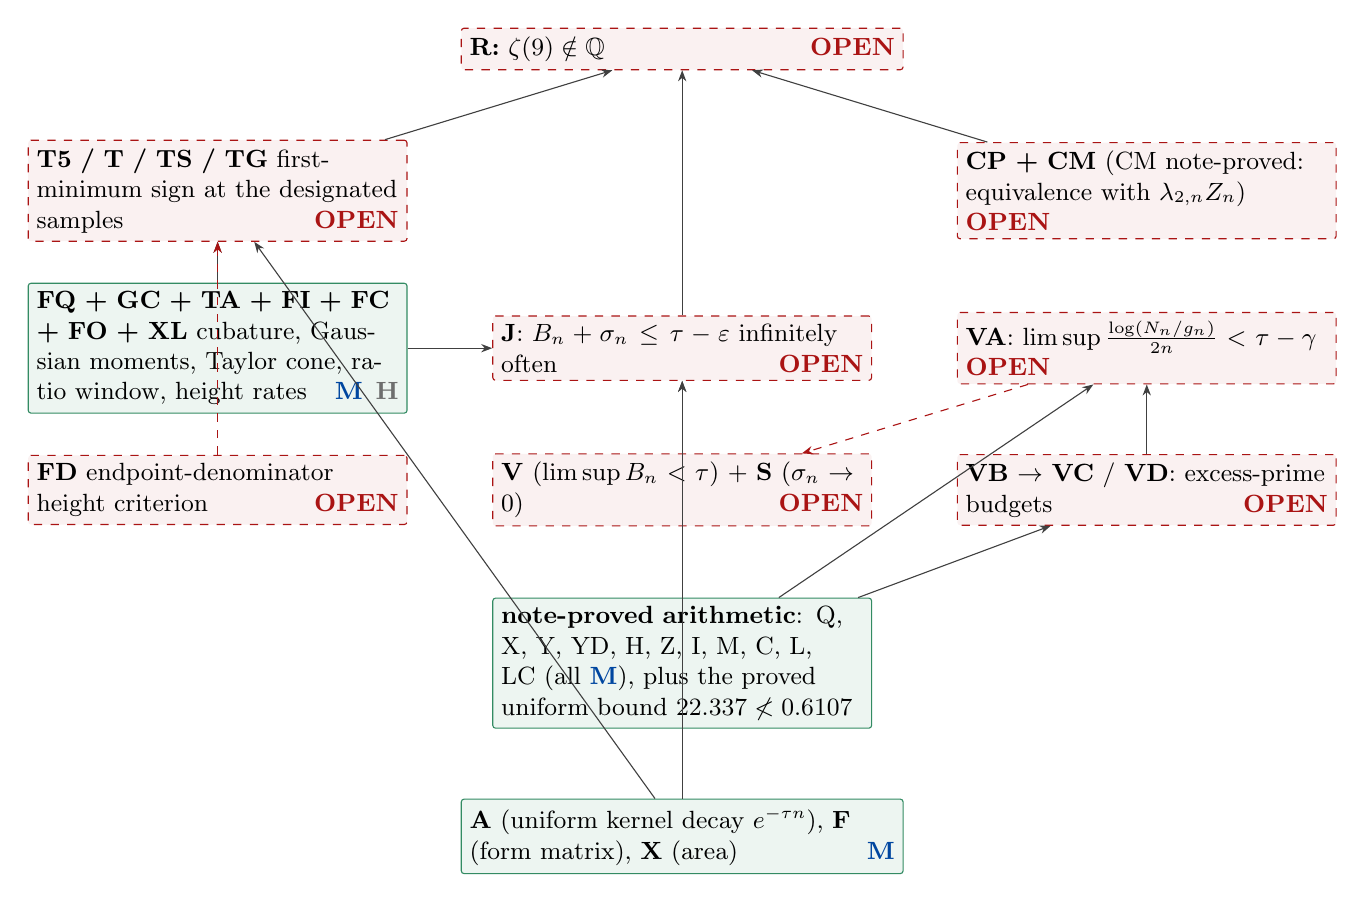
\begin{tikzpicture}[
  font=\small,
  box/.style={draw, rounded corners=1pt, inner sep=3pt, align=left},
  ok/.style={box, draw=okgreen!80, fill=okgreen!7},
  gap/.style={box, draw=gapred, dashed, fill=gapred!6},
  ar/.style={-{Stealth[length=4pt]}, draw=black!75},
  mr/.style={-{Stealth[length=4pt]}, draw=gapred, dashed}
]
\node[gap, text width=5.4cm] (R) at (7.5, 11.2) {\textbf{R: $\zeta(9)\notin\Q$} \hfill \stO};
\node[gap, text width=4.6cm] (CPCM) at (13.4, 9.4) {\textbf{CP + CM} (CM note-proved: equivalence with $\lambda_{2,n}Z_n$) \hfill \stO};
\node[gap, text width=4.6cm] (T5) at (1.6, 9.4) {\textbf{T5 / T / TS / TG} first-minimum sign at the designated samples \hfill \stO};
\node[ok, text width=4.6cm] (FQ) at (1.6, 7.4) {\textbf{FQ + GC + TA + FI + FC + FO + XL} cubature, Gaussian moments, Taylor cone, ratio window, height rates \hfill \stM\, \stH};
\node[gap, text width=4.6cm] (FD) at (1.6, 5.6) {\textbf{FD} endpoint-denominator height criterion \hfill \stO};
\node[gap, text width=4.6cm] (J) at (7.5, 7.4) {\textbf{J}: $B_n+\sigma_n\le\tau-\varepsilon$ infinitely often \hfill \stO};
\node[gap, text width=4.6cm] (VS) at (7.5, 5.6) {\textbf{V} ($\limsup B_n<\tau$) + \textbf{S} ($\sigma_n\to0$) \hfill \stO};
\node[gap, text width=4.6cm] (VA) at (13.4, 7.4) {\textbf{VA}: $\limsup\frac{\log(N_n/g_n)}{2n}<\tau-\gamma$ \hfill \stO};
\node[gap, text width=4.6cm] (VB) at (13.4, 5.6) {\textbf{VB} $\to$ \textbf{VC} / \textbf{VD}: excess-prime budgets \hfill \stO};
\node[ok, text width=4.6cm] (notes) at (7.5, 3.4) {\textbf{note-proved arithmetic}: Q, X, Y, YD, H, Z, I, M, C, L, LC (all \stM), plus the proved uniform bound $22.337 \not< 0.6107$};
\node[ok, text width=5.4cm] (A) at (7.5, 1.2) {\textbf{A} (uniform kernel decay $e^{-\tau n}$), \textbf{F} (form matrix), \textbf{X} (area) \hfill \stM};
\draw[ar] (T5) -- (R);
\draw[ar] (CPCM) -- (R);
\draw[ar] (FQ) -- (T5);
\draw[mr] (FD) -- (T5);
\draw[ar] (J) -- (R);
\draw[ar] (VS) -- (J);
\draw[mr] (VA) -- (VS);
\draw[ar] (VB) -- (VA);
\draw[ar] (FQ) -- (J);
\draw[ar] (A) -- (T5);
\draw[ar] (A) -- (J);
\draw[ar] (notes) -- (VB);
\draw[ar] (notes) -- (VA);
\end{tikzpicture}
\end{center}

\section{The Prove2me platform layer}
\label{sec:platform}

The local DAG was partially wired into a \emph{private} Prove2me mission. Everything below is
read back from receipts in \texttt{roadmap/platform/}; none of it changes the mathematical status.

\begin{longtable}{@{}p{0.30\textwidth}p{0.66\textwidth}@{}}
\toprule \textbf{Item} & \textbf{Identifier / status} \\ \midrule
\endfirsthead
\toprule \textbf{Item} & \textbf{Identifier / status} \\ \midrule
\endhead
proposal / mission & \texttt{06faf23f-00c2-4edf-92ab-1212cdb7d7d6} /
    \texttt{8195d8fe-059f-4515-92b4-57b585e2bac6}, status \texttt{Private},
    \texttt{is\_live\_private\_mission}: true \\
root theorem & \texttt{ZetaNine.irrational\_zeta\_nine} = \texttt{523f37b8-ae98-\dots}, read back
    \stO \\
original items & Zudilin's four-value disjunction \texttt{a925cba9}; two-form criterion
    \texttt{207cc87c}; abstract margin bridge \texttt{cbb9cc51} \\
accepted general reductions & \texttt{irrational\_of\_two\_small\_integer\_forms} and
    \texttt{exponential\_margin\_of\_volume\_and\_shape} --- full proofs, compiled locally with Lean
    4.33.1, platform status \texttt{ACCEPTED} \\
accepted abstract cores & \texttt{volume\_baseline\_cancellation} (\texttt{d6b0eb73}),
    \texttt{finite\_prime\_budget} (\texttt{8496d3a0}),
    \texttt{finite\_prime\_discount} (\texttt{0f7bb5e3}) --- all \texttt{ACCEPTED} \\
wired 2026-09-25 & \texttt{irrational\_of\_small\_nonzero\_integer\_forms} (\texttt{c1147ec6},
    \stR{} Proved), \texttt{taylor\_sign\_implies\_kernel\_sum\_pos} (\texttt{a8a15e54}, \stR{}),
    \texttt{quadrature\_exact\_of\_moments} (\texttt{443fb397}, \stR{}),
    \texttt{exponentially\_small\_nonzero\_forms\_of\_zeta\_nine} (\texttt{60c1cf49}, \stO{}),
    \texttt{exponentially\_small\_independent\_forms\_of\_zeta\_nine} (\texttt{691b1665}, \stO{}) \\
root decompositions & \texttt{42bd3e13} (one-form: criterion + open obligation) and \texttt{0da22fdd}
    (two-form), both \texttt{SKETCH\_ACCEPTED} \\
milestones & 40 (was 35); 32 research milestones read back, with IDs in
    \texttt{platform/new-results-receipt.json} \\
blind readback & all five newly wired statements returned \emph{faithful and well-posed} \\
\bottomrule
\end{longtable}

\paragraph{What is deliberately not wired, and why.} The receipts and
\texttt{wiring/README.md} record two constraints: (i) a child that only says ``there exist small
integer forms'' is \emph{equivalent} to the root once a criterion is available --- a disguised
restatement, not a decomposition; the two obligations now on the root therefore pin a \emph{fixed
exponential rate} and are stated to be strictly stronger than the root. (ii) A parent with free
parameters cannot import a closed child theorem, so a multi-level graph needs a definition layer
first. Consequently the concrete quantities of the roadmap ($F_n$, $K_n$, Smith data, weighted
areas, congruence-lattice minima) have \emph{no Lean definitions}, and no arithmetic arrow
($V\leftarrow VA,Q,X$; $VA\leftarrow VB,Y$; $VB\leftarrow VC,H,Z$) was published as a platform
decomposition. The note-proved layer (F, A, G, P, M, C, L, X, H, Z, I, LC, TP) is explicitly
\emph{not} presented as platform-proved.

\section{Additional gaps found in Part II}
\label{sec:gaps2}

\begin{itemize}[leftmargin=1.4em]
\item \textbf{G8.1 (classification hygiene).} ``Note-proved'' is not ``proved'' in the sense used for
      Part I's \stR, and it is not ``Lean-proved''. Of $40$ roadmap nodes, $27$ are note-proved and
      $13$ open; the platform holds $8$ theorem-level proofs (two general reductions, three abstract
      cores, three wired lemmas) with \emph{abstract} statements. Nothing in the corpus justifies
      quoting a note-proved node as established.
\item \textbf{G8.2 (abstract vs.\ concrete).} The three accepted abstract cores are conditional
      (``given the concrete area identity'', ``for the concrete valuation inequality'', ``for the
      concrete discount identity''). The concrete instances are exactly the unformalised parts. An
      accepted abstract proof therefore does \emph{not} discharge the corresponding local node; the
      mapping table \texttt{new-dag-mapping.md} says so.
\item \textbf{G8.3 (reductions to strictly stronger statements).} The two root decompositions are
      sound but one-directional: the obligations are strictly stronger than the target, hence the
      reduction cannot be reversed. Combined with CM (an equivalence), the honest global picture is:
      the root is equivalent to a critical-scale statement (CM/CP) and is \emph{implied} by several
      stronger statements (J; T5/T/TS/TG; V$\wedge$S), none of which is proved.
\item \textbf{G8.4 (FQ/T5 activation threshold --- new finding of this audit).} The five designated
      samples of FQ are $k_{n,j}=\lfloor nx_*+j\sqrt{n/a}+\frac12\rfloor$. Because
      $\sqrt{n/a}\asymp0.19\sqrt{n}$ while $n(x_*-1)\approx0.00298n$, the five points become distinct
      \emph{and} all lie in the summation range $k>n$ only for $n\gtrsim1686$: recomputation gives
      $k_{12,j}\equiv12$ (all five equal), $k_{192,j}=\{191,192,193,193,194\}$ (not distinct; one
      point $\le n$, where $R_n$ vanishes), $k_{384,j}=\{383,\dots,387\}$ (distinct but $383<n$),
      $k_{1400,j}=\{1400,1402,\dots,1408\}$ ($=n$), and only from $n=2000$ on
      ($\{2001,2003,2006,2008,2011\}$) does every point exceed $n$. \emph{Consequence:} the finite
      parameters used anywhere in the mission ($n\le384$; $n\le192$ in rounds 5--7) cannot exercise
      FQ or T5 at all, so no finite regression in the corpus tests the newest route. The roadmap's
      wording (``for sufficiently large $n$'') is correct; the finite evidence base does not reach it.
\item \textbf{G8.4b (quantitative, and checked independently for this audit).} Going beyond the
      vacuity question: solving the exact five-point system for the \emph{true} kernel moments in the
      standardised variable gives weights that are \emph{not} all positive at $n=1000$ and $n=2000$,
      and only become positive at $n=6000$ and $n=20000$ (table below). The failure at $n=2000$
      persists when the nodes are placed at their ideal real positions, so it is not an
      integer-rounding artefact but a genuine consequence of the slow moment convergence: the true
      standardised moments are $(1,0.235,1.056,0.964,3.630)$ at $n=6000$ and
      $(1,0.129,1.017,0.523,3.188)$ at $n=20000$, against the Gaussian $(1,0,1,0,3)$, and the
      deviation decays only like $n^{-1/2}$ (measured ratio $0.2355\to0.1290$ over a factor $3.33$ in
      $n$, versus the predicted $3.33^{-1/2}=0.548$). With \emph{Gaussian} moments substituted at the
      same nodes the weights are positive at every tested $n$, and the control
      (nodes $-2..2$, Gaussian moments) reproduces $(1/12,1/6,1/2,1/6,1/12)$ exactly. So the
      mechanism is sound and FQ's ``eventually'' is plausible; what is quantitatively clear is that
      the positivity threshold lies above $2000$ and the weights are still $\sim0.04$ away from the
      claimed limit at $n=20000$. \textbf{Caution for anyone reproducing this:} the weight system
      must be solved in the standardised variable $s$ (nodes near $-2..2$); solving it in $u$ (nodes
      near $y_*=2.0089$ with a $10^{-3}$ spread, Vandermonde condition number $\approx10^{13}$) returns
      meaningless numbers even at $60$ digits.
\item \textbf{G8.4c (what the corpus actually certifies here).} The mission's own
      \texttt{check\_gaussian\_five\_point.py} verifies (i) the exact rational five-point table
      $(-2,-1,0,1,2;1/12,1/6,1/2,1/6,1/12)$ against $(1,0,1,0,3)$ and (ii) the rational interval
      $330.658<a<330.659$, $\sqrt{3/a}\in(0.095251,0.095252)$. It does \emph{not} compute the true
      kernel's moments or the actual weights at any $n$. Hence GC's moment limit and FQ's positivity
      rest on their prose proofs alone --- the finite certificate covers the limit constant, not the
      convergence.
\item \textbf{G8.5 (graph typing).} In \texttt{DAG.md} the root emits solid edges to ingredient nodes
      ($X$, $A$, $F$, $G$, $Q$, $Y$, $M$, $C$, \dots). Those are inputs, not sufficient conditions;
      only the composite groups in the prose (``T5 $\wedge$ FQ $\wedge$ X $\wedge$ A $\wedge$ F
      $\Rightarrow$ R'') are real reductions. The prose is right; the edge types are not, and an
      undeclared node id (\texttt{TC}) appears once as a source. Purely presentational, but a reader
      who reads the graph alone would over-count the reductions.
\item \textbf{G8.6 (bookkeeping).} \texttt{proposal-receipt.json} still records
      \texttt{reviewed\_docs\_version: 0.10.9} although the platform moved to $0.11.1$ and the local
      version guard was updated; the receipt is therefore not a full record of the current review
      state.
\item \textbf{G8.7 (the threshold slack is real but tiny).} The route needs $-f_*>0$; the proved
      statement is $-f_*<-\tau$, i.e.\ the decay exceeds the requirement by
      $10.5641538\ldots-10.564=1.54\times10^{-4}$ per unit $n$ (recomputed independently below). It
      is a genuine proof with a genuine, very small margin, and every downstream statement inherits
      that margin.
\item \textbf{G8.8 (unclosed uniformity, restated).} Every closing statement in the roadmap is a
      $\forall$: ``for every primitive $z$'' (S), ``for infinitely many even $n$'' (J, T5, T, TS, TG,
      FD), ``along all even $n$'' (V, VA, VB, VC, VD). The corpus contains five-scale finite
      certificates for each and states in every case that they do not imply the $\forall$. This is
      the same wall as in Part I, in a new coordinate system.
\end{itemize}

\section{Independent checks for Part II}
\label{sec:checks2}

Recomputed from the construction itself (\texttt{R\_n(t)=n!^7(t-n)\_n(t+n+1)\_n/Q\_n(t)^9}), without
using the mission's scripts. Scripts and transcripts:
\texttt{missions/zeta9/verification/audit-2026-09-25/} (files \texttt{roadmap\_layer\_check.py},
\texttt{fq\_gc\_check2.py} and their \texttt{*\_out.txt}).

\begin{longtable}{@{}p{0.055\textwidth}p{0.55\textwidth}p{0.35\textwidth}@{}}
\toprule \textbf{Check} & \textbf{What was recomputed} & \textbf{Result} \\ \midrule
\endfirsthead
\toprule \textbf{Check} & \textbf{What was recomputed} & \textbf{Result} \\ \midrule
\endhead
A10 & The saddle of the round-5--7 family: $f(x)=10x\log x-(x-1)\log(x-1)+(x+2)\log(x+2)
      -10(x+1)\log(x+1)$ (derived here from the construction), its critical point, $f(x_*)$ and
      $a=-f''(x_*)$. & $x_*=1.00297646575489808$, $f(x_*)=-10.5641538376402$,
      $a=330.65816828687$, $\sqrt{3/a}=0.09525131927$, $y_*=2.00893825661$. These reproduce the
      notes' values exactly: round-2's $x_*\approx1.00297646575$ and rate $-10.5641538376$;
      round-7's $-10.564155<f_*<-10.564$; GC's $330.658<a<330.659$ and
      $0.095251<\sqrt{3/a}<0.095252$. \stN \\
A11 & The FQ sample points $k_{n,j}$ for $n=12,24,48,96,192,384,1000,1400,2000,4000$: distinctness
      and membership in $k>n$. & Degenerate for all $n\le1400$; the first $n$ with five distinct
      points all exceeding $n$ is $2000$. See G8.4/G8.4b. \\
A12 & The five-point cubature from the true kernel moments: standardised moments $E[s^e]$, $e=0..4$,
      and the exact weights, at $n=1000,2000,6000,20000$; plus the Gaussian control. & Control
      (nodes $-2..2$, Gaussian moments) $=(1/12,1/6,1/2,1/6,1/12)$ exactly. True weights:
      $(0.0553,-0.2045,1.1434,-0.7731,0.7789)$ (n=1000, not positive),
      $(0.0412,0.0027,0.7287,-0.0107,0.2381)$ (n=2000, not positive),
      $(0.0435,0.1207,0.6049,0.0280,0.2029)$ (n=6000, positive),
      $(0.0568,0.1717,0.5174,0.1246,0.1295)$ (n=20000, positive). Moment deviations from Gaussian
      decay like $n^{-1/2}$. See G8.4b. \stN \\
\bottomrule
\end{longtable}

\noindent\textbf{Scope.} A10 confirms the constants that the entire post-round-7 programme is built
on, to full displayed precision. A11 and A12 are quantitative statements about \emph{when} the
newest lemmas start to say anything; neither contradicts the lemmas as stated (both are ``for all
sufficiently large $n$'' statements) and neither closes any open node. Nothing here was used to
adjust any claim in the corpus.

\section{Consolidated closure list (both layers)}
\label{sec:closure2}

Nothing in Part I or Part II is closed into an irrationality proof. For completeness, the full list
of what would be needed:

\begin{enumerate}[leftmargin=1.6em]
\item[\textbf{C1}] an asymptotic (or matching lower bound) for the true primitive multiplier of the
      Part I family (T4);
\item[\textbf{C2}] a lower bound for $|L_{n,m}|$, e.g.\ a phased saddle main term with
      non-cancellation (T3, incl.\ the branch issue in $\Phi'_\alpha+2\pi i=0$);
\item[\textbf{C3}] $A_{n,m}\ne0$ on the Part I range (T1);
\item[\textbf{C4}] the assembly $0<|P_{n,m}(\zeta(9))|\le e^{-cn}$ along an infinite sequence (T5 of Part I);
\item[\textbf{C5}] the Gram-branch uniformity, the independently certified potential constant, and
      the $\zeta(9)$ normalisation cost (T6);
\item[\textbf{C6}] Lean definitions for $F_n$, $K_n$, the Smith data, the weighted area and the
      congruence-lattice minima --- without them the roadmap's obligations cannot even be
      \emph{stated} faithfully on the platform;
\item[\textbf{C7}] one of the geometric nodes T5 / T / TS / TG / FD (equivalently, in the critical
      scale of CM: CP), together with the formalisation of the note-proved layer FQ, GC, TA, FI, FC,
      FO, XL, TP, SP, CM;
\item[\textbf{C8}] one of the arithmetic nodes J / V$\wedge$S, hence VA, VB, VC or VD, whose proved
      uniform estimate still stands at $22.337$ against a requirement of $0.61071437$;
\item[\textbf{C9}] a uniform statement in \emph{any} of the above over an infinite set of parameters
      --- the single missing ingredient common to all nine rounds;
\item[\textbf{C10}] formal verification of the note-proved layer ($27$ roadmap nodes plus the Part I
      note proofs); today only eight abstract platform theorems exist.
\end{enumerate}

\section{Consequence: no irrationality claim}
\label{sec:conclusion}

\textbf{Unconditional statement.} Because T1--T4 and T6 are open, and because T3/T4 are not merely
unproved but have \emph{no mechanism} in the audited corpus (an upper bound on $|L|$ cannot be
sharpened into a lower bound; a proved multiplier cannot be sharpened into a statement about
$m_{\mathrm{prim}}$), the audited material \emph{cannot} be combined into a proof that $\zeta(9)$ is
irrational, nor into a proof that it is rational, nor into a proof that this family of constructions
fails. \textbf{No proof of irrationality is claimed here}. The same holds for the later layers: of
the roadmap's $40$ nodes $13$ are open and none of the $27$ note-proved ones is Lean-checked; the
platform's two root decompositions accept obligations that are \emph{strictly stronger than} (and not
equivalent to) the root, and the concrete objects those obligations are about have no Lean
definitions. Nothing has been repaired to make the dependencies close: the DAGs have red edges, in
both layers, and they remain red.

\textbf{Closure list.} \S\ref{sec:closure2} gives the canonical list C1--C10, and none of the ten is
closed. C1--C5 are the Part~I obligations (an asymptotic or matching lower bound for the true
primitive denominator $m_{\mathrm{prim}}$; a lower bound for $|L_{n,m}|$; $A_{n,m}\ne0$; the assembly
$0<|P_{n,m}(\zeta(9))|\le e^{-cn}$ along an infinite sequence; and the Gram-branch package of
uniformity, an independently certified potential constant and the $\zeta(9)$ normalization cost).
C6--C10 are the Part~II obligations (Lean definitions for $F_n,K_n$, Smith data, weighted areas and
congruence minima; one of the geometric nodes T5/T/TS/TG/FD or CP; one of the arithmetic nodes J or
$V\wedge S$ via VA/VB/VC/VD, whose proved uniform estimate still stands at $22.337$ against a required
$0.61071437$; a uniform statement over an infinite parameter set, which is the single ingredient
missing in all nine rounds; and formalization of the note-proved layer).

\textbf{What may be quoted from the effort.} From Part I: the exact algebra and the
reflection/partial-fraction identities (R1--R6); the two integerization theorems and their relation
(R7--R10); the exact and large-prime valuation formulas (R11--R12); the multiplier asymptotics and the
$\Gamma$-enclosure method (R13--R17); the exact contour identity and kernel facts (R18--R19); the
phase and its exact $n\log n$ cancellation, the certified upper bound
$\limsup\frac1n\log|L|\le\sup H_\alpha$ with its six certified constants (R20--R26); the finite
sample records and their certificates (R27--R30, R37--R38); and, with the two caveats flagged, the
Gram positivity/degree facts (R31--R32) and the moment-integrality and rank lemma (R34--R35). From
Part II: the all-$n$ leading-coefficient nonvanishing theorem (round~4); the connection theorem and
determinant closed form (round~7); the proved exponents $f_*<-10.564$ and $\gamma=\frac14\log
3\,711\,015\,000$ (independently reproduced, A10); the note-proved identities Q, X, Y, YD, H, Z
\emph{as note-proved}; and the four proved \emph{negative} results (GO, FM, and the two frozen-model
obstructions) \emph{only} in their stated scopes. Each of these should be quoted with its status tag,
and \emph{not} as a step toward irrationality.

\textbf{Artifacts.} Part I: \texttt{missions/zeta9/\{status.md, report.md\}},
\texttt{research/\{analytic.md, arithmetic.md, linear-experiments.md\}},
\texttt{verification/\{summary.json, linear-results.jsonl, linear-coeff/, linear-audit.json,
independent-audit.json, arithmetic-certificates.json, arithmetic-improved-certificates.json,
analytic-vertical-bound.json, gram-results.jsonl, gram-manifest.json,
gram-arithmetic-certificates.json, artifact-manifest.json\}}, and
\texttt{missions/zeta7/\{status.md, research/analytic-foundations.md\}}. Part II:
\texttt{missions/zeta9/roadmap/\{DAG.md, dag.json, research/, verification/\}},
\texttt{missions/zeta9/round2/\dots round9/}, and
\texttt{missions/zeta9/roadmap/platform/\{README.md, proposal-receipt.json,
new-results-receipt.json, wiring/wiring-receipt.json, wiring/README.md\}}.
Audit scripts and transcripts: \texttt{missions/zeta9/verification/audit-2026-09-25/}.

\end{document}
